% TPI de Simulacion - Informe final
% Compilar con:  latexmk -pdf informe-final.tex   (desde la carpeta del informe)

\documentclass{article}

\usepackage{arxiv}

\usepackage[utf8]{inputenc}
\usepackage[T1]{fontenc}
\usepackage[spanish,es-tabla]{babel}
\usepackage{enumitem}       % sin esto babel-spanish rompe los itemize con argumento opcional
\usepackage{hyperref}
\usepackage{url}
\usepackage{booktabs}
\usepackage{tabularx}
\usepackage{amsfonts}
\usepackage{microtype}
\usepackage{graphicx}
\usepackage{amsmath,amssymb}
\usepackage{float}
\usepackage{caption}
\usepackage{array}
\usepackage{multirow}

\graphicspath{{figuras/}}
\captionsetup{font=small,labelfont=bf,skip=6pt}

\renewcommand{\topfraction}{0.88}
\renewcommand{\bottomfraction}{0.70}
\renewcommand{\textfraction}{0.12}
\renewcommand{\floatpagefraction}{0.80}
\raggedbottom

\newcolumntype{L}{>{\raggedright\arraybackslash}X}
\newcolumntype{R}{>{\raggedleft\arraybackslash}X}
\setlist{nosep}
\setlength{\tabcolsep}{4pt}

% encabezado de una sola línea (el título completo ocupaba dos y se pisaba con el texto)
\renewcommand{\shorttitle}{Impacto de la Línea F sobre la red de Subte de Buenos Aires}

% enlaces del trabajo: repositorio y los dos modelos publicados en AnyLogic Cloud
\newcommand{\enlaceRepositorio}{\url{https://github.com/BrunoNeirotti/TPI-Simulacion}}
\newcommand{\enlaceCloudRed}{\url{https://cloud.anylogic.com/model/0bfb3484-d911-409e-bf99-d3563ca6d44a}}
\newcommand{\enlaceCloudEstacion}{\url{https://cloud.anylogic.com/model/ea098342-e565-4808-b7ab-12621b2f76b4}}

% el estilo arxiv escribe «Abstract»
\renewenvironment{abstract}
{\centerline{\large\bfseries\scshape Resumen}\begin{quote}}
{\end{quote}}

\title{Evaluación mediante simulación del impacto de la Línea F sobre la operación de la red de Subte de la Ciudad de Buenos Aires\\[1ex]\large Informe final del Trabajo Práctico Integrador de Simulación}

\author{
  \textbf{Bruno Neirotti}\textsuperscript{1} \qquad \textbf{Alexis Galasco}\textsuperscript{2} \qquad \textbf{Tomás Salami}\textsuperscript{3} \qquad \textbf{Giani Mesapelle}\textsuperscript{4} \qquad \textbf{Francisco Lovatti}\textsuperscript{5} \\[0.5ex]
  \textsuperscript{1}Legajo: 47792 -- \texttt{bneirotti@gmail.com} \\
  \textsuperscript{2}Legajo: 51474 -- \texttt{alexis.galasco123@gmail.com} \\
  \textsuperscript{3}Legajo: 51534 -- \texttt{tomas.salami1@gmail.com} \\
  \textsuperscript{4}Legajo: 52897 -- \texttt{gianimesapelle04@gmail.com} \\
  \textsuperscript{5}Legajo: 52420 -- \texttt{franciscolovatti08@gmail.com} \\[0.5ex]
  Universidad Tecnológica Nacional -- FRRo \\
  Zeballos 1341, S2000, Argentina \\
}
\date{Noviembre de 2026\\[1.5ex]
  \small Modelos, planilla de resultados y fuentes oficiales: \enlaceRepositorio \\[0.5ex]
  Modelos para correr en el navegador (AnyLogic Cloud): \\
  red de Subte: \enlaceCloudRed \\
  estación Constitución en 3D: \enlaceCloudEstacion}

\begin{document}
\maketitle

\begin{abstract}
La Línea F de Subte, hoy en licitación, tiene un objetivo oficial: descongestionar la Línea C. Este trabajo
mide si lo cumple. Se construyó en AnyLogic un modelo de simulación de toda la red de Subte de la Ciudad de
Buenos Aires (seis líneas, 90 estaciones, 14 combinaciones) que sigue a cada pasajero y a cada tren durante un
día hábil completo, alimentado con datos públicos y con la matriz de viajes entre estaciones que Subterráneos
de Buenos Aires (SBASE) entregó por pedido de acceso a la información. El modelo reproduce la carga de
pasajeros por tramo que mide SBASE con un error medio del 8\,\%. Después se le agregó la Línea F con la traza
y los parámetros de su proyecto oficial, y se simuló cien veces cada escenario para separar el efecto real del
azar; cada resultado se da con su intervalo de confianza del 95\,\%. Resultado: la Línea F cumple su
objetivo. La carga máxima de la Línea C cae un 54,7 $\pm$ 0,4\,\%, a menos de la mitad, cualquiera sea la
frecuencia con que circule la nueva línea. Para la red en conjunto la mejora es menor: el viaje medio baja
44,8 $\pm$ 0,6 s (4\,\%) y la espera 11,6 $\pm$ 0,6 s, porque cuatro de cada cinco viajes no cambian de
ruta. La Línea F lleva 8.134 $\pm$ 17 pasajeros por hora en su tramo más cargado, con los trenes a poco más
de la mitad de su capacidad.
Un segundo modelo, de la estación Constitución de la Línea F construida sobre los planos oficiales, muestra
que la estación absorbe las dos horas pico sin que se formen colas crecientes: un pasajero tarda menos de tres
minutos entre que entra y sube al tren.
\end{abstract}

% =====================================================================
\section{Introducción}

La Línea F es una obra real. Su traza fue fijada por la Ley 670 de la Ciudad en 2001 [12], el proyecto
ejecutivo se licitó en 2026 con un presupuesto oficial de 1.350 millones de dólares, su Estudio de Impacto
Ambiental pasó por audiencia pública en agosto de 2026 y el servicio está previsto para 2031. La
documentación oficial le asigna un objetivo: descongestionar la Línea C, que en Constitución recibe a buena
parte de los pasajeros que llegan desde el sur por el ferrocarril Roca. Pero ningún documento del proyecto
compara cómo funcionaría la red con y sin la nueva línea: ni qué tramos se alivian, ni cuánto, ni con qué
frecuencia de trenes.

Este trabajo hace esa comparación con un modelo de simulación. La propuesta se presentó en agosto de 2026
[1]; este informe cuenta qué se construyó, qué resultados dio y cuáles son sus límites. La
sección~\ref{sec:objetivos} fija los objetivos y cómo se mide el resultado; la~\ref{sec:metodologia}
describe el sistema, los datos, los modelos, cómo se comprobaron y cómo se planificaron las corridas; la~\ref{sec:resultados}
compara la red con y sin la Línea F, y la~\ref{sec:conclusiones} responde a los objetivos y señala los límites del
trabajo. El anexo resume los supuestos de los modelos.

Todo el trabajo se apoya en datos oficiales. Cuando un dato no existe, el informe lo dice; cuando hubo que
suponer algo, se explica el supuesto y, siempre que se pudo, se midió cuánto cambia el resultado si el
supuesto fuera otro.

\paragraph{Términos que se usan.} La tabla~\ref{tab:terminos} explica los términos técnicos que aparecen a lo
largo del informe.

\begin{table}[htbp]
  \centering\small
  \caption{Términos técnicos del informe.}
  \label{tab:terminos}
  \begin{tabularx}{\linewidth}{>{\bfseries\raggedright\arraybackslash}p{0.27\linewidth}L}
    \toprule
    Simulación de eventos discretos & El modelo avanza de un suceso al siguiente (entra un pasajero, llega
      un tren, sale un tren) en lugar de avanzar en pasos fijos de tiempo. \\
    Agente & Cada pasajero y cada tren del modelo, con sus propios datos: origen, destino y ruta; línea,
      posición y pasajeros a bordo. \\
    Réplica & Una simulación completa del día con otra secuencia de números al azar. Se hacen cien por
      escenario para ver cuánto del resultado es efecto real y cuánto es azar. \\
    Intervalo de confianza del 95\,\% & El margen ($\pm$) que acompaña a una media, calculado como indica
      Ross [20] (sección~\ref{sec:diseno}): con 95\,\% de confianza el valor verdadero está dentro de ese
      rango, porque el procedimiento acierta 95 de cada 100 veces. Si el intervalo de la diferencia entre dos
      escenarios no incluye el cero, la diferencia no es casual. \\
    Intervalo entre trenes & Tiempo entre dos trenes seguidos de la misma línea y sentido. \\
    Carga por tramo & Pasajeros que viajan a bordo entre dos estaciones consecutivas en una hora. \\
    Matriz origen--destino & Tabla con la cantidad de viajes de cada estación a cada otra. \\
    Verificar, calibrar, validar & Verificar es comprobar que el modelo hace lo que se diseñó. Calibrar es
      ajustar un parámetro hasta que el modelo reproduce un dato. Validar es comparar el modelo con un dato
      \emph{distinto} del usado para calibrar. \\
    \bottomrule
  \end{tabularx}
\end{table}

% =====================================================================
\section{Objetivos}
\label{sec:objetivos}

\textbf{Objetivo general.} Medir con un modelo de simulación, construido en AnyLogic y alimentado con datos
oficiales, cómo cambia la operación de la red de Subte cuando se agrega la Línea F, y en particular si la
nueva línea cumple su objetivo oficial: descongestionar la Línea C.

\textbf{Objetivos específicos.}
\begin{enumerate}
  \item Construir un modelo de la red actual en el que cada pasajero y cada tren son agentes, para un día hábil
    completo, y comprobar que reproduce la carga de pasajeros que mide SBASE.
  \item Agregar la Línea F con la traza y los parámetros de su proyecto, sin indicarle al modelo cuántos
    pasajeros la usan: cada pasajero recalcula su ruta más rápida sobre la red nueva y el reparto resulta de
    eso. Comparar la red con y sin la nueva línea.
  \item Medir cuánto depende el resultado de la frecuencia de la Línea F, que el proyecto no define.
  \item Comprobar, con un submodelo peatonal hecho sobre los planos del proyecto, si la estación Constitución
    de la Línea F mueve a sus pasajeros en las dos horas pico.
\end{enumerate}

\textbf{Cómo se mide el resultado.} Para la red: el tiempo medio de viaje, desde que el pasajero entra hasta
que sale; la espera media en los andenes; los pasajeros por hora en el tramo más cargado de la Línea C y de la
Línea F, y qué tan llenos van los trenes. Para la estación Constitución: el tiempo desde la entrada hasta el
tren, el tiempo desde el tren hasta la salida y la cantidad de personas que quedan adentro al terminar la
hora pico, que indica si las colas crecen.

\textbf{Alcance.} Un día hábil, de 5 a 24 h; las seis líneas de Subte, sin el Premetro; la demanda actual,
sin las personas que empezarían a usar el Subte por la nueva línea; y un solo escenario futuro, con la Línea F
completa.

% =====================================================================
\section{Metodología}
\label{sec:metodologia}

Esta sección describe el sistema que se simula, de dónde salen los datos, cómo se construyeron los dos
modelos, cómo se comprobó que son correctos y cómo se planificaron las corridas. Los supuestos se pusieron
por escrito y se discutieron en el grupo antes de programar cada parte; el anexo los resume.

\subsection{El caso: la red actual y la Línea F}
\label{sec:caso}

\subsubsection{La red en operación}

La red tiene seis líneas (A, B, C, D, E y H), 90 estaciones contando por separado cada línea de una
combinación, y 14 estaciones de combinación. Es radial: las líneas A, B, D y E llegan al centro desde el
oeste y la C y la H las cruzan de norte a sur. Según SBASE, en un día hábil de septiembre de 2024 se hicieron
827.976 viajes. La hora pico concentra el 9,9\,\% de los ingresos del día y pasa un tren cada 3,15 min en la
Línea C (la más frecuente) y cada 5,22 min en la E. El tramo más cargado de toda la red es el de la Línea C
entre San Juan y Retiro, de 8 a 9 h: según el modelo, 12.436 $\pm$ 64 pasajeros por hora, con los trenes al
74\,\% de su capacidad.

\subsubsection{La Línea F}

Lo que sigue sale del expediente ambiental [10], del pliego de licitación [11] y de las respuestas oficiales
a los pedidos de acceso a la información [9]. No se usan cifras de prensa.

\begin{figure}[htbp]
  \centering
  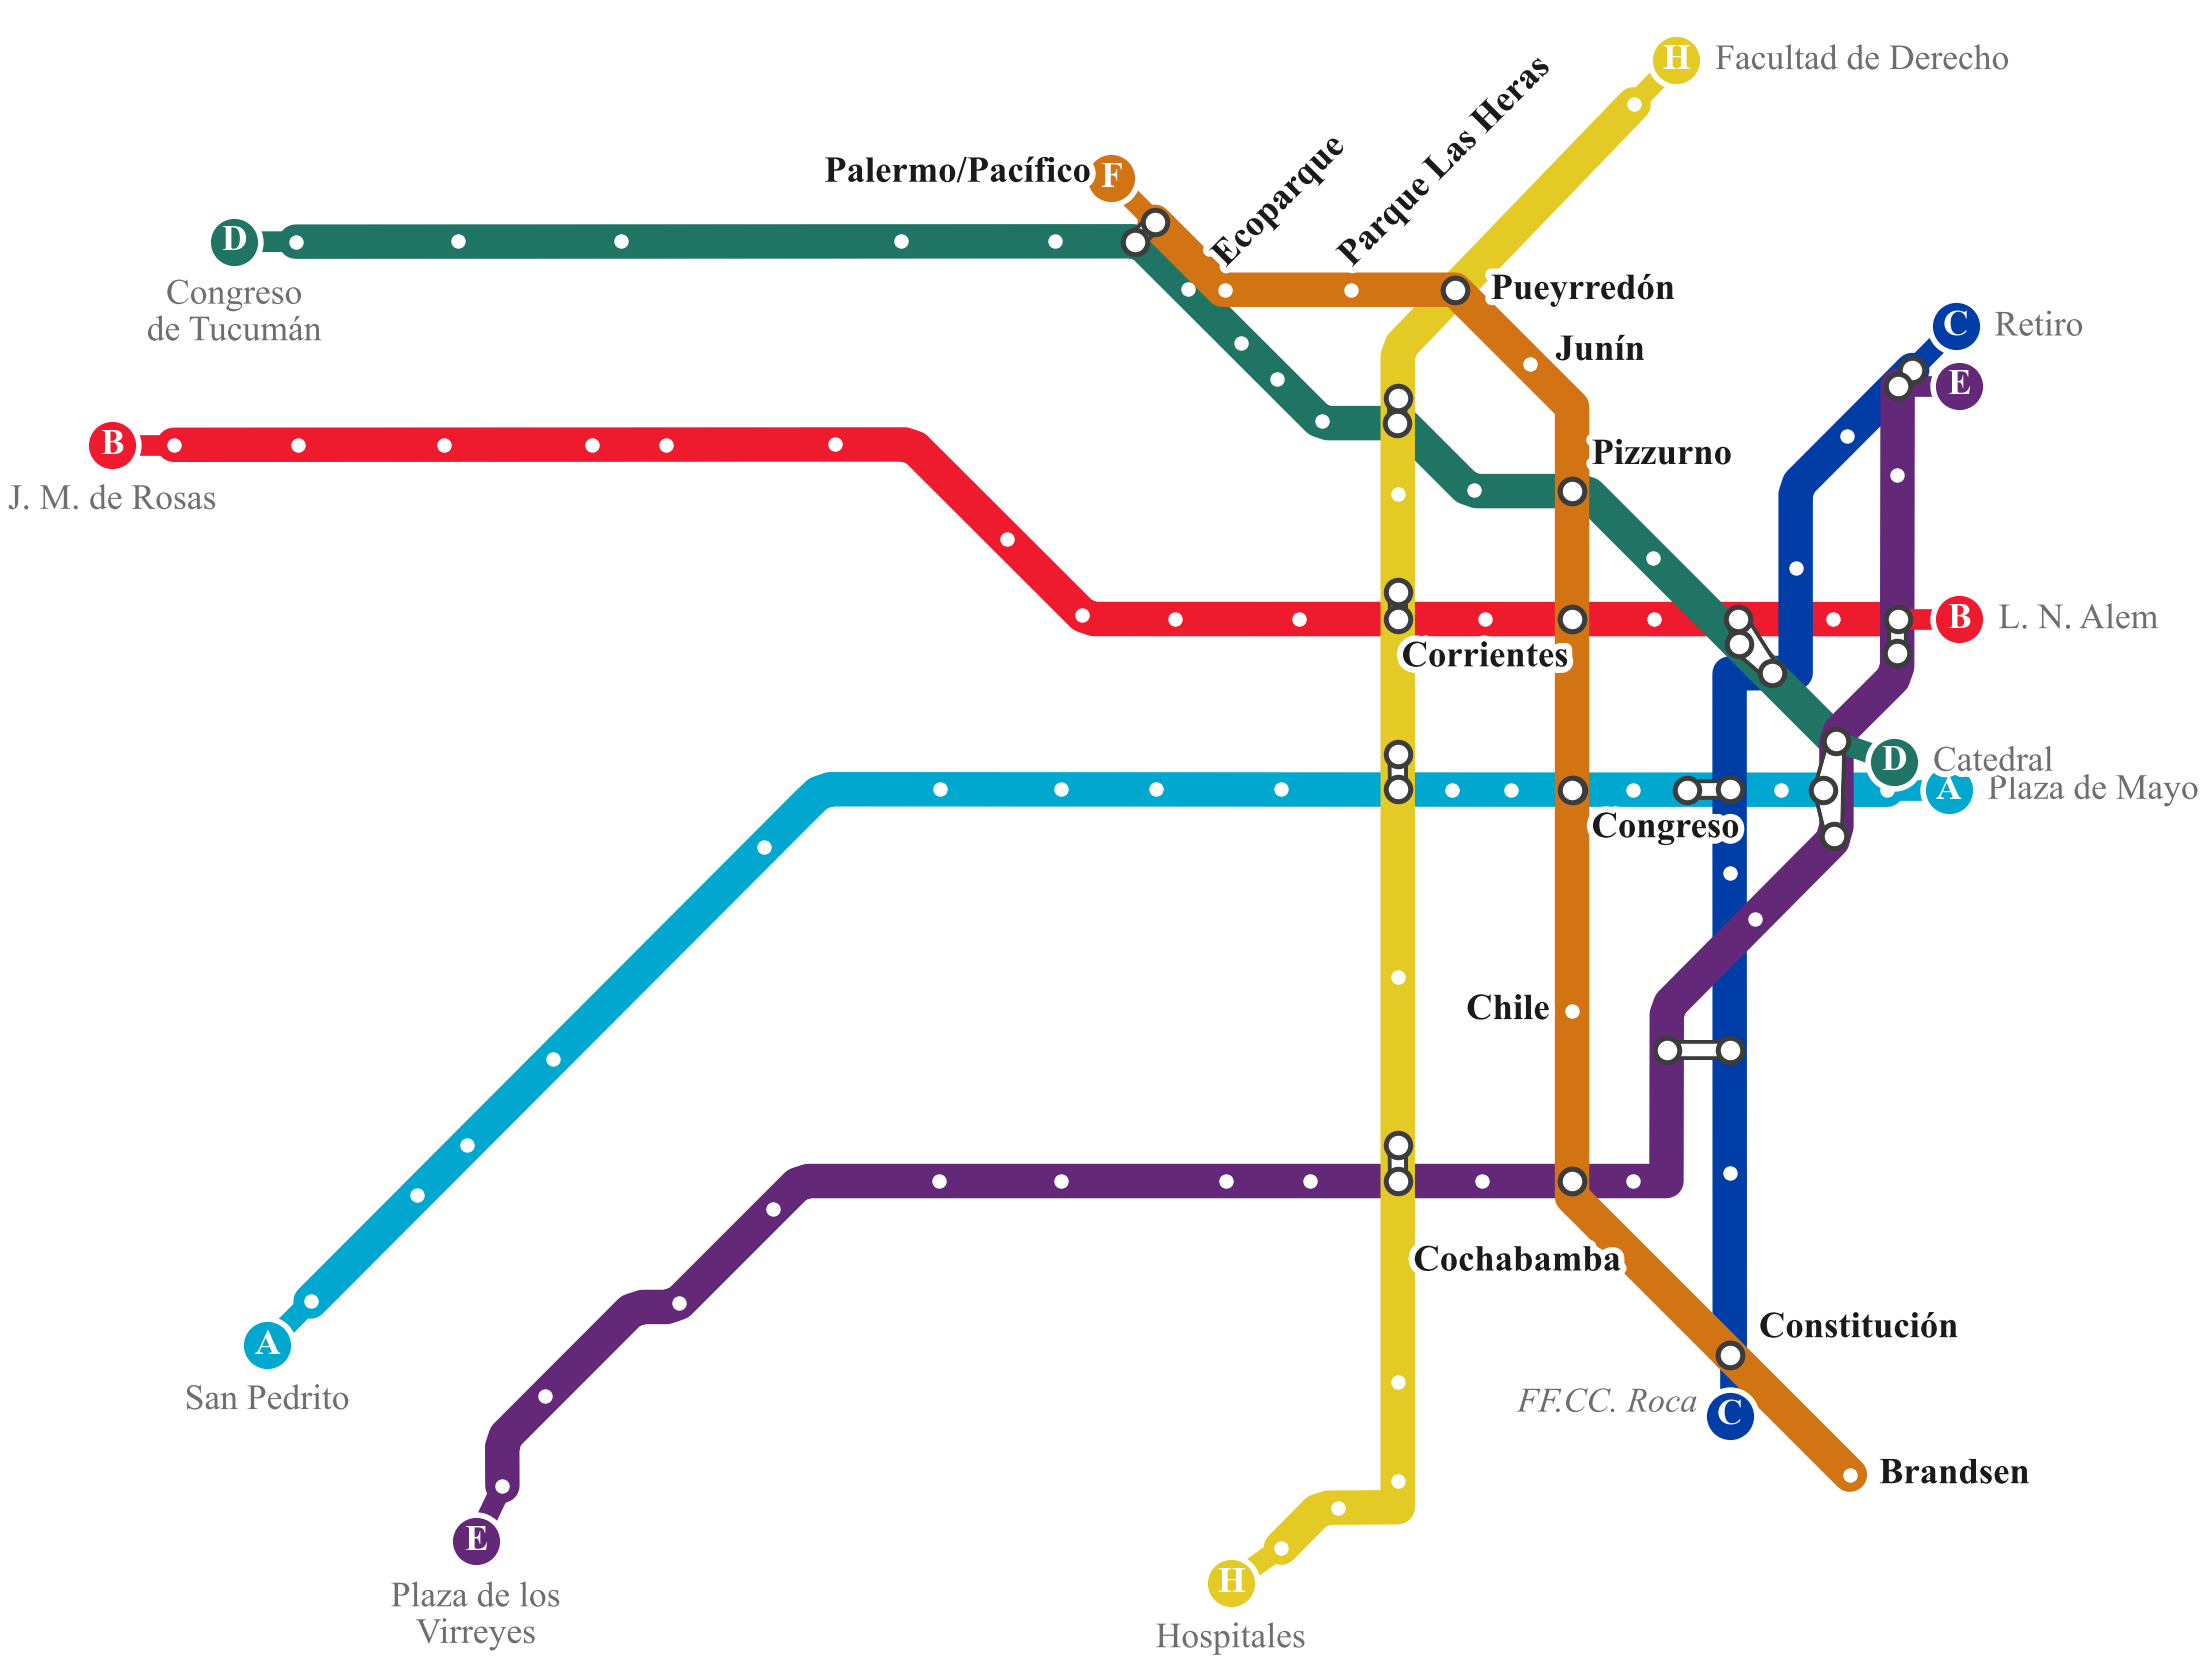
\includegraphics[width=0.95\linewidth]{red-y-linea-f.png}
  \caption{La red de Subte con la Línea F (en naranja) entre Brandsen y Palermo/Pacífico. Las seis líneas en
  operación siguen el mapa de red oficial de EMOVA [22]; la F se dibujó con las mismas reglas, por las
  avenidas de su traza. Los círculos con borde oscuro son estaciones de combinación, unidas por un pasillo
  blanco.}
  \label{fig:red}
\end{figure}

\begin{itemize}
  \item \textbf{Traza.} Doce estaciones entre Barracas y Palermo, en 9,8 km (figura~\ref{fig:red}):
    Brandsen, Constitución, Cochabamba, Chile, Congreso, Corrientes, Pizzurno, Junín, Pueyrredón, Parque Las
    Heras, Ecoparque y Palermo/Pacífico. Combina con las seis líneas existentes y con los ferrocarriles Roca
    y San Martín.
  \item \textbf{Parámetros de diseño.} Trenes de seis coches para 1.075 pasajeros, un tren cada 90 s (o cada
    100 s «de requerirse»), 30 s de detención por estación, 25 trenes en total y 18 min de viaje de punta a
    punta.
  \item \textbf{No hay plan de servicio.} El Ministerio de Movilidad e Infraestructura informó que la
    frecuencia la decidirá el futuro operador. Por eso este trabajo no fija una frecuencia para la Línea F:
    prueba varias.
  \item \textbf{Se habilita entera, en una sola etapa}, de Brandsen a Palermo. Hay entonces un solo escenario
    futuro.
  \item \textbf{El objetivo declarado es aliviar la Línea C}, que según el propio expediente lleva un 70\,\%
    de viajes que combinan con el ferrocarril. El plan de expansión PETERS [13] ya planteaba la Línea F como
    la alternativa para que la C opere sin congestión.
\end{itemize}

\subsubsection{La demanda prevista de la Línea F}

No existe una previsión oficial confiable de cuántos pasajeros llevará la Línea F. Hay dos cifras y no
pueden ser ciertas a la vez. Un estudio de SBASE de 2019 prevé unos 73.900 pasajeros en la hora pico, y la
comunicación oficial anuncia entre 270.000 y 300.000 por día. Para que las dos coincidieran, la Línea F
tendría que recibir en una sola hora el 25\,\% de sus pasajeros del día; la red actual recibe el 9,9\,\%.
Además, el estudio de 2019 analizó una traza distinta de la actual, de 13 estaciones. Por eso este trabajo
no usa ninguna de las dos cifras como dato de entrada: la demanda de la Línea F la calcula el propio modelo
(sección~\ref{sec:escenario}), y la previsión de 2019 se usa solo para comparar.

% =====================================================================
\subsection{Fuentes de datos y preparación}
\label{sec:datos}

Casi ningún dato que el modelo necesita estaba publicado listo para usar. Prepararlos fue buena parte del
trabajo: cada paso se programó por separado y deja un informe de control. Esta sección resume de dónde sale
cada dato y qué problemas hubo que resolver.

\subsubsection{Fuentes}

\begin{description}[style=nextline,leftmargin=1.5em]
  \item[{Recorridos y tiempos: GTFS de Subte [6].}] El archivo oficial de horarios en formato GTFS da el
    orden de las estaciones de cada línea, el tiempo de viaje entre estaciones y el tiempo mínimo para
    combinar. Tiene dos defectos que el modelo corrige: el tiempo de detención es un valor fijo de 24 s en
    todas las estaciones (de diseño, no medido), y en un sentido de la Línea E los tiempos estaban mal
    cargados; se reemplazaron por los del sentido contrario.
  \item[{Pasajeros que entran: Viajes Molinetes [4].}] Pasajeros por molinete, estación y cuarto de hora:
    206,6 millones de ingresos en 2025. Se usaron solo los días hábiles normales, sin paros ni días
    atípicos.
  \item[{Trenes: Trenes despachados [5].}] La hora de salida de cada tren desde cada cabecera. De ahí se midió
    el intervalo real entre trenes por línea, cabecera y hora, sobre 663.709 intervalos.
  \item[{Destinos: Viajes y etapas del AMBA [7, 8].}] La única fuente abierta que dice adónde va cada
    pasajero, para un día de octubre de 2024. Se usó para repartir los viajes a lo largo del día.
  \item[{Matriz de viajes y carga por tramo de SBASE [9].}] Llegaron por pedido de acceso a la información:
    la matriz de viajes entre las 90 estaciones de un día hábil de septiembre de 2024 (y de sus dos horas
    pico), y los pasajeros a bordo por tramo de las seis líneas en las dos horas pico. Es el dato que más
    cambió el trabajo: dio la demanda real y, por primera vez, un dato observado contra el cual comprobar el
    modelo.
  \item[{La Línea F: expediente ambiental, pliego y respuestas oficiales.}] Traza, estaciones, distancias y
    parámetros operativos.
\end{description}

\subsubsection{Del dato crudo a lo que usa el modelo}

\begin{enumerate}
  \item \textbf{Estaciones y red.} Se unificaron los nombres de las 90 estaciones entre las cuatro fuentes y
    se armó la red como un grafo: 90 estaciones, 166 tramos y 28 pasillos de combinación.
  \item \textbf{Rutas.} Para cada par de estaciones se calculó la ruta más rápida, sumando los tiempos de
    viaje, las paradas intermedias, las combinaciones y una penalización por cada transbordo que representa
    la espera del tren siguiente y la incomodidad de cambiar de línea. Cada pasajero usa esa ruta (asignación «todo o nada» [3]). El 22\,\%
    de los pares viaja directo, el 48\,\% hace un transbordo y el 30\,\% dos.
  \item \textbf{La penalización por transbordo.} Se probaron valores de 0 a 300 s y se midió cuál reproduce
    mejor la carga por tramo de SBASE en la hora pico de la mañana. Todos los valores entre 30 y 300 s dan
    prácticamente el mismo error (entre 6,3 y 6,5\,\%): el dato solo descarta los menores de 30 s. Se usaron
    120 s, la mitad del intervalo medio entre trenes en hora pico, que es lo que espera en promedio quien
    llega al andén sin mirar el horario.
  \item \textbf{Demanda.} La cantidad de viajes y su reparto entre estaciones salen de la matriz de SBASE:
    827.289 viajes en el día. Las horas pico reproducen exactamente las matrices de SBASE; el resto del día
    se reparte con el perfil horario de la encuesta de destinos y los cuartos de hora con los molinetes.
  \item \textbf{Trenes.} Se ajustó una distribución de probabilidad al intervalo entre trenes de cada línea,
    cabecera y hora (227 casos), como se vio en la materia:
    \begin{itemize}
      \item Se compararon cinco distribuciones teóricas por máxima verosimilitud. El \emph{criterio de
        Akaike}, que elige la que mejor describe los datos penalizando los parámetros de más, prefirió la
        lognormal en 181 de los 227 casos (figura~\ref{fig:ajuste}).
      \item Los trenes salen con bastante regularidad: el coeficiente de variación del intervalo es 0,28. Un
        \emph{proceso de Poisson}, en el que los trenes saldrían totalmente al azar, tendría 1; suponerlo
        habría exagerado las esperas.
      \item Las pruebas de bondad de ajuste rechazaron todas las distribuciones teóricas en la mayoría de los
        casos. Es lo esperable con más de mil datos por caso: con tanta información, las pruebas detectan
        cualquier diferencia, por chica que sea. Además, la Línea H tiene dos intervalos típicos (cerca de
        205 y de 290 s) que ninguna distribución teórica reproduce.
    \end{itemize}
    Por eso el modelo usa la \textbf{distribución empírica}: sortea los intervalos directamente de los
    datos observados, con el método de Law [2]. Se comprobó con la distancia de \emph{Kolmogorov--Smirnov},
    que mide la mayor diferencia entre la distribución del modelo y la de los datos: 0,012, es decir, nunca
    más de 1,2 puntos porcentuales. Los datos de ajuste son de julio a diciembre de 2025 y se verificaron con
    marzo a mayo de 2026.
\end{enumerate}

\begin{figure}[htbp]
  \centering
  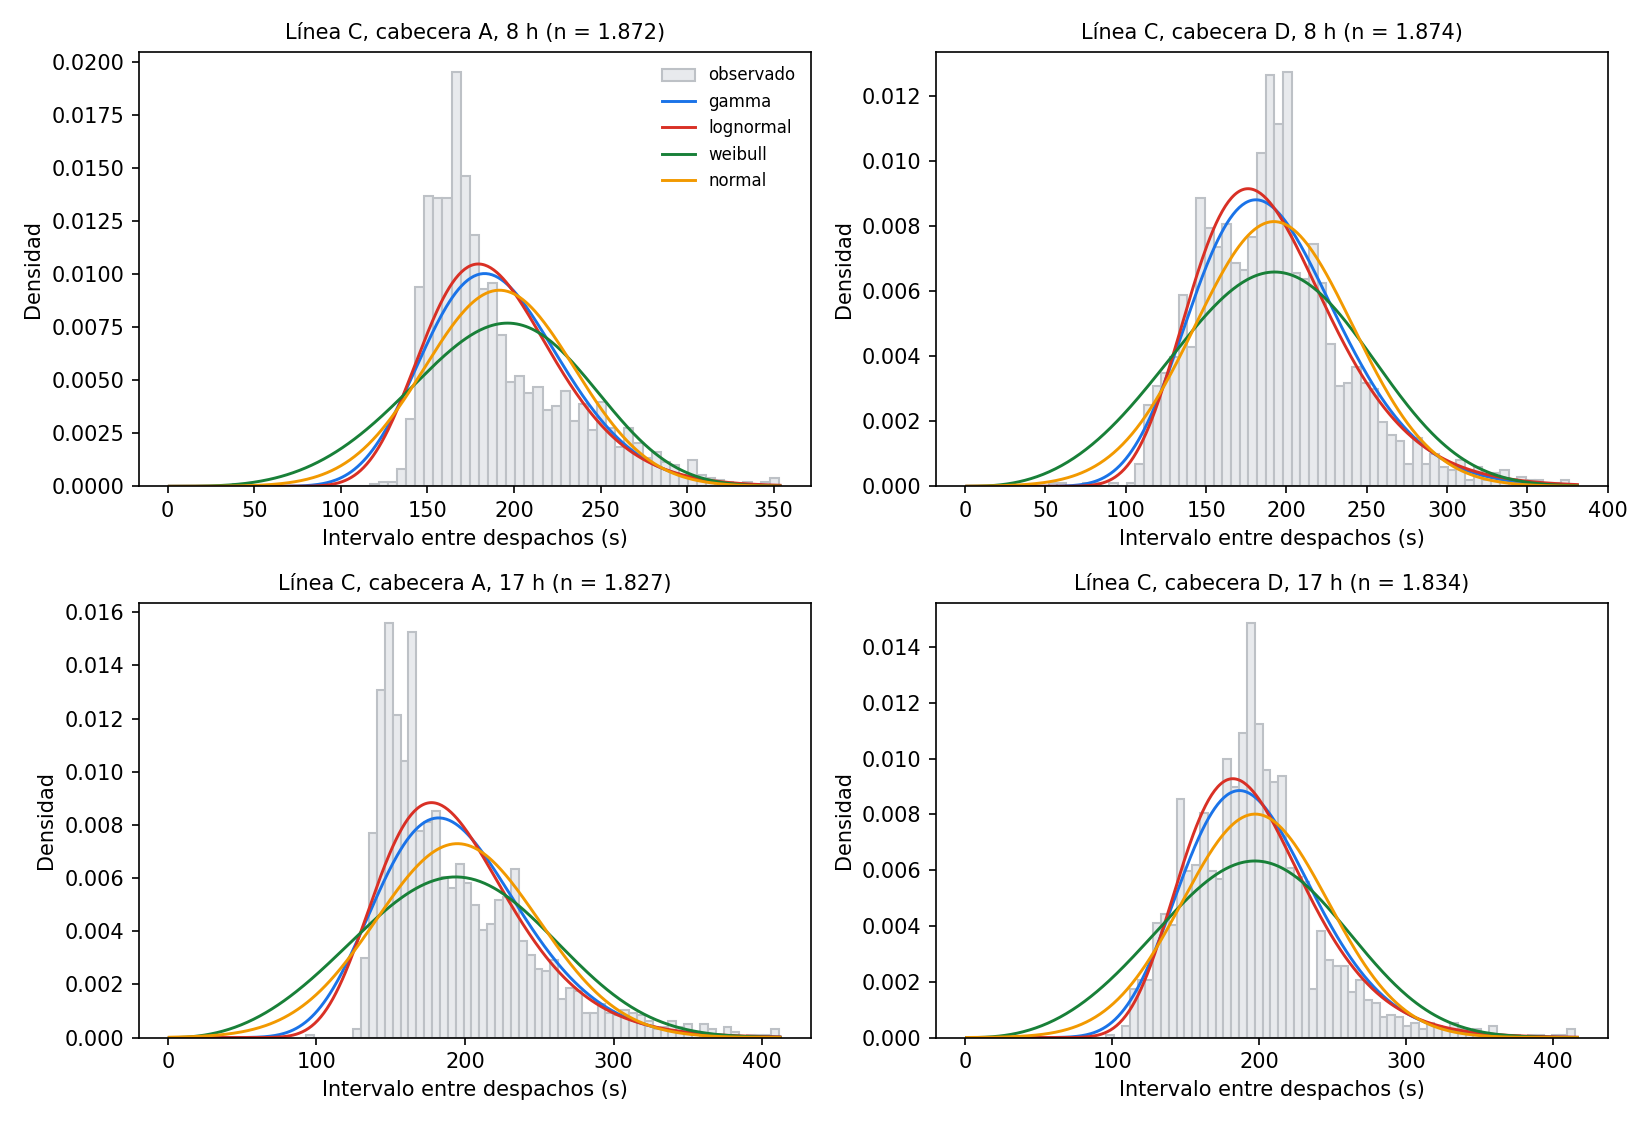
\includegraphics[width=0.85\linewidth]{ajuste-intervalos-c-pico.png}
  \caption{Intervalo entre trenes de la Línea C en hora pico, por cabecera. Las barras son los datos y las
  curvas, las distribuciones teóricas ajustadas. Ninguna curva sigue bien a los datos, que tienen varios
  picos; por eso el modelo sortea directamente de los datos observados.}
  \label{fig:ajuste}
\end{figure}

% =====================================================================
\subsection{El modelo de la red}
\label{sec:modelo}

\subsubsection{Los límites de la licencia}

El modelo corre en AnyLogic 8.9 Personal Learning Edition [19], la versión gratuita para estudiantes. Antes
de diseñarlo se midieron sus límites con modelos de prueba, porque la documentación no los precisa. Tres
resultados definieron el diseño:
\begin{itemize}
  \item La versión limita la simulación a cinco horas, pero los bloques de la Process Modeling Library
    quedan exentos: un modelo hecho con ellos corrió veinte horas. Por eso todo el modelo se arma con esa
    biblioteca, y puede simular el día completo.
  \item La versión no permite crear más de 50.000 agentes por corrida, y el día tiene más de 800.000 viajes. Pero los
    agentes de una población declarada de antemano no cuentan para ese límite. Por eso los pasajeros salen
    de una población fija de 32.000 que se reutiliza: cuando un pasajero termina su viaje, vuelve a la
    población y sale de nuevo como otro. Como mucho hay unos 29.000 pasajeros en la red a la vez, así que alcanza.
  \item Cada tipo de agente admite 200 bloques, y no alcanzan para dibujar un diagrama por estación. Por eso
    un solo par de diagramas de flujo sirve para todas, y la red (estaciones, tramos, rutas) se lee de tablas
    de datos.
\end{itemize}

\subsubsection{Agentes y flujos}

El modelo tiene tres tipos de agente. \texttt{Main} representa la red: carga las tablas, mantiene una cola
de espera por andén y lleva los contadores. \texttt{Pasajero} guarda su origen, destino, hora de entrada y
ruta. \texttt{Formacion}, que es un tren (hay 150), guarda su línea, sentido, capacidad, posición y los
pasajeros a bordo.

\begin{figure}[htbp]
  \centering
  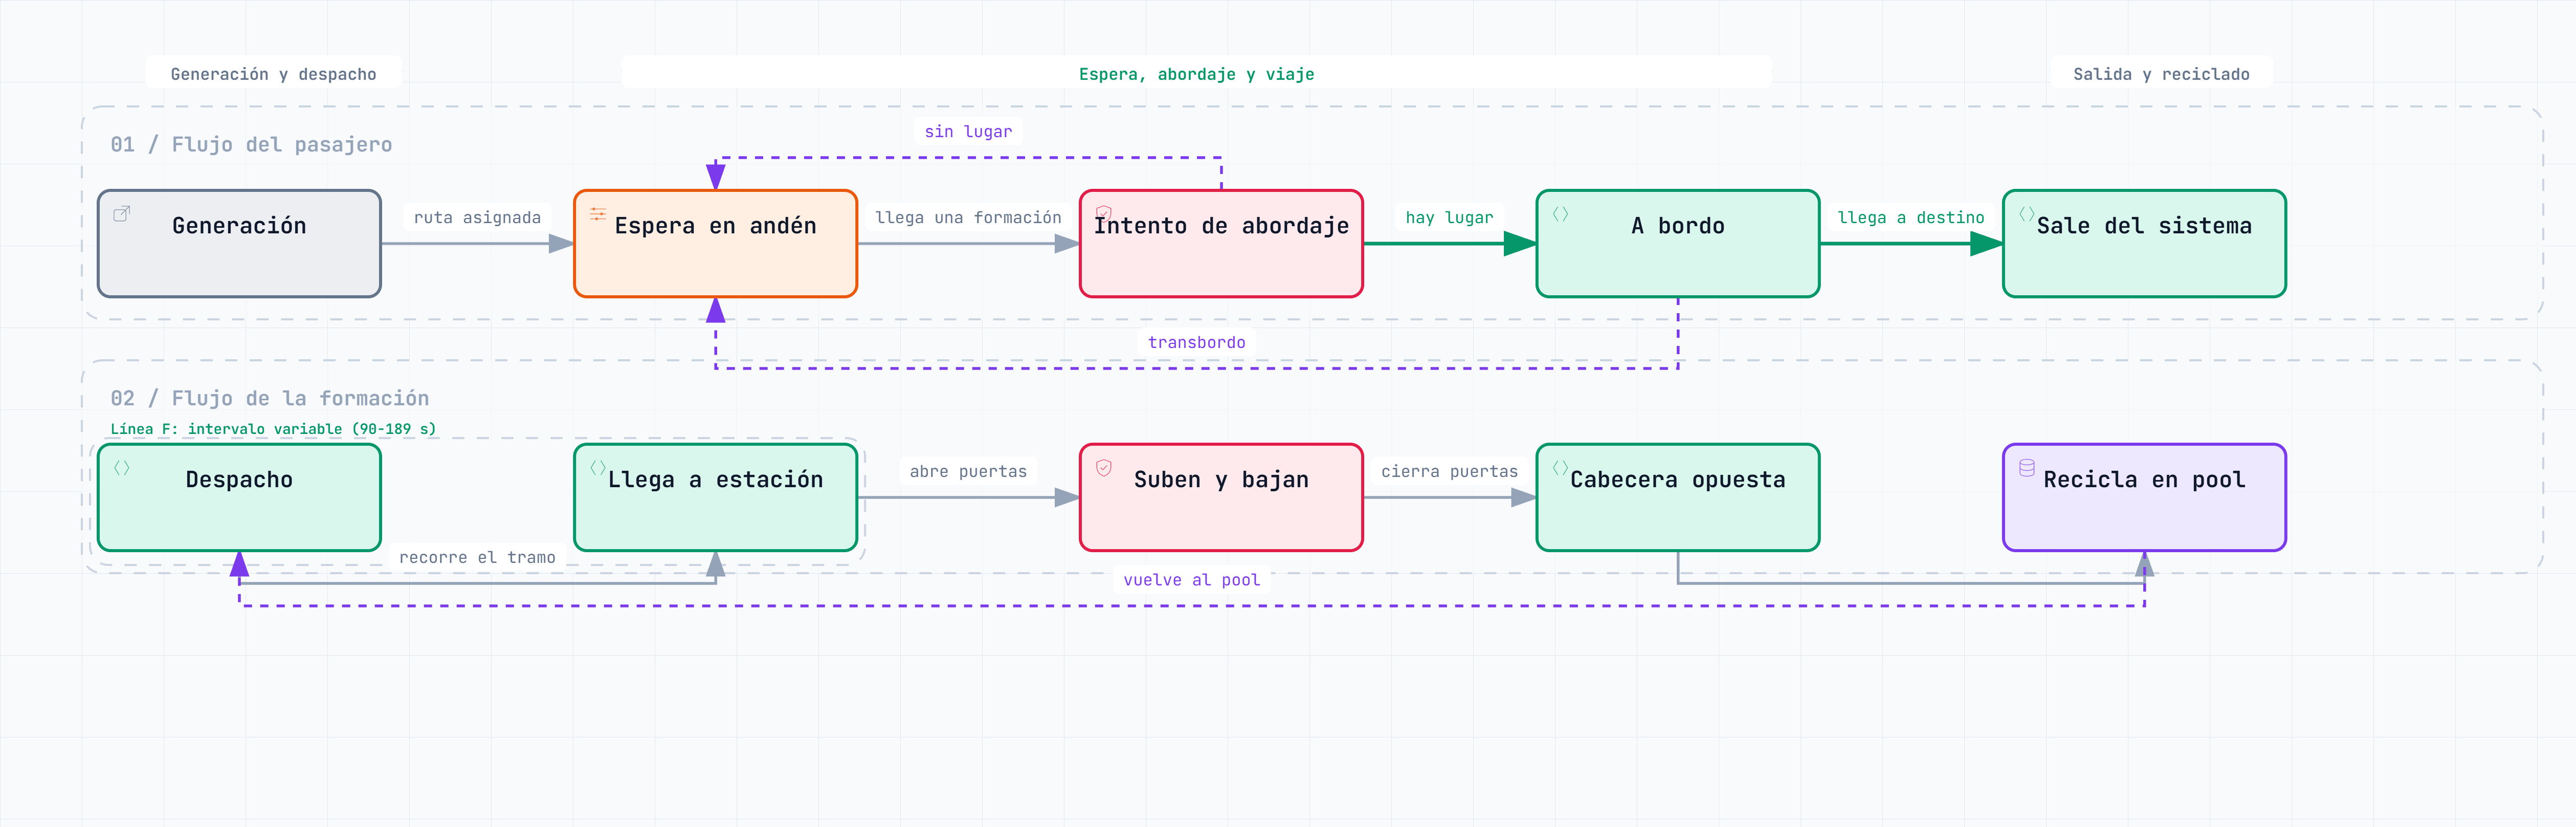
\includegraphics[width=\linewidth]{diagrama-conceptual-modelo.png}
  \caption{Arriba, el recorrido del pasajero; abajo, el del tren. El pasajero espera en el andén hasta que
  un tren lo sube, y viaja hasta que el tren lo baja en la estación de su ruta; si tiene que combinar,
  camina el pasillo y vuelve a esperar. El tren sale de la cabecera, recorre cada tramo, se detiene en cada
  estación para bajar y subir gente, y al llegar a la otra punta vuelve a la reserva. Cada diagrama tiene seis
  bloques y sirve para las 90 estaciones.}
  \label{fig:flujos}
\end{figure}

La figura~\ref{fig:flujos} muestra los dos diagramas de flujo. Todo lo dispara el tren: al llegar a una
estación baja a los pasajeros que terminan ahí o combinan, y al salir sube, por orden de llegada, a los que
esperan, hasta llenarse. Quien no entra se queda en el andén y espera el tren siguiente.

\subsubsection{Cómo llegan los pasajeros y cómo salen los trenes}

\textbf{Pasajeros.} Llegan según un proceso de Poisson no homogéneo: al azar, pero con una tasa que cambia
cada cuarto de hora según la matriz de viajes. Al entrar, cada pasajero sortea su destino según los viajes
de su estación a esa hora y toma la ruta más rápida.

\textbf{Trenes.} Cada cabecera despacha sus trenes por separado, con intervalos sorteados de la
distribución empírica de su línea y hora. A las 5:30, cuando abre el servicio, los trenes arrancan desde las
mismas estaciones intermedias desde las que arrancan en la realidad.

\textbf{Detención.} El tiempo que el tren pasa en cada estación depende de cuánta gente baja y sube: un
mínimo de 24 s (30 s en la Línea F) más 1,85 s por cada pasajero que baja y 2,1 s por cada uno que sube,
repartidos entre las puertas, según el manual de capacidad de transporte TCQSM [14]. Un tren no entra a un
tramo hasta que el anterior lo dejó libre, como en la realidad. La capacidad de cada tren es la cantidad de
coches de su línea (5 o 6) por 179 pasajeros por coche.

\subsubsection{Cómo se usa el modelo}

El modelo es un único proyecto de AnyLogic. Un parámetro, \texttt{escenario}, elige qué red se simula: la
actual o la red con la Línea F a cada una de las frecuencias que se prueban. Tiene dos experimentos: uno que
simula el día cien veces y muestra los histogramas del tiempo de viaje, de la espera y de los transbordos, y
otro que recorre la red actual y las cinco frecuencias de la Línea F, diez días cada una. Los datos que lee
viajan con el modelo, en su propia carpeta. El modelo se puede correr en el navegador, sin instalar AnyLogic,
desde AnyLogic Cloud, eligiendo el escenario; lo mismo la estación Constitución en 3D
(sección~\ref{sec:peatonal}). Los enlaces están en la portada, junto con el del repositorio que reúne los
modelos, la planilla con los resultados de todas las corridas y las fuentes oficiales del trabajo. La lógica que no se resuelve con bloques (las colas por andén
y la lectura de las rutas) está escrita como clases Java dentro del mismo proyecto.

% =====================================================================
\subsection{Verificación y validación}
\label{sec:verificacion}

\subsubsection{Verificación: el modelo hace lo que se diseñó}

\textbf{No se pierden pasajeros.} En todas las corridas, los pasajeros que entraron son exactamente los que
llegaron a destino más los que siguen viajando al final del día.

\textbf{La carga coincide con el cálculo directo.} Si se cargan los viajes sobre sus rutas sin simular, se
obtiene una carga por tramo que la simulación debe reproducir. La reproduce: correlación 0,999 en la hora pico
de la mañana y 1,000 en la de la tarde, con diferencias de 3,2 y 2,7\,\%. La coincidencia no es exacta, y no
debe serlo: el cálculo directo pone cada viaje en su hora de salida, y la simulación lo pone en cada tramo a la
hora en que el tren pasa de verdad.

\textbf{Un segundo programa da lo mismo.} Como herramienta de control, se escribió aparte un simulador con la
misma lógica en Java, sin AnyLogic. Si los dos programas, hechos por separado, dan el mismo resultado con los
mismos datos, es muy improbable que compartan un error. La tabla~\ref{tab:cruzada} muestra que coinciden
dentro del margen del azar, con y sin la Línea F. El simulador de control corre un día en menos de un
segundo; por eso se usó también para las corridas de la sección~\ref{sec:resultados} que requieren muchas
repeticiones.

\begin{table}[htbp]
  \centering\small
  \caption{AnyLogic contra el simulador de control, con los mismos datos. Media e intervalo de confianza del
  95\,\%, cien réplicas en cada caso. El pico de la Línea C es la mayor carga de pasajeros por hora en un
  tramo: AnyLogic promedia el pico de cada réplica y el control toma el tramo y la hora de mayor carga
  media, por eso AnyLogic da un poco más; en los dos es el tramo que sale de San Juan hacia Retiro, de 8 a 9 h.}
  \label{tab:cruzada}
  \begin{tabular}{lrrrr}
    \toprule
    & \multicolumn{2}{c}{Red actual} & \multicolumn{2}{c}{Con la Línea F cada 100 s} \\
    \cmidrule(lr){2-3}\cmidrule(lr){4-5}
    Indicador & AnyLogic & Control & AnyLogic & Control \\
    \midrule
    Tiempo medio de viaje (s) & 1.110,8 $\pm$ 0,4 & 1.110,7 $\pm$ 0,4 & 1.065,4 $\pm$ 0,4 & 1.065,9 $\pm$ 0,4 \\
    Espera media por viaje (s) & 188,5 $\pm$ 0,4 & 188,5 $\pm$ 0,4 & 176,5 $\pm$ 0,4 & 176,9 $\pm$ 0,4 \\
    Trenes que toma cada pasajero & 1,443 & 1,443 & 1,466 & 1,466 \\
    Pico de la Línea C (pas./h) & 12.463 $\pm$ 55 & 12.436 $\pm$ 64 & 5.694 $\pm$ 27 & 5.639 $\pm$ 37 \\
    \bottomrule
  \end{tabular}
\end{table}

\textbf{Los extremos también coinciden.} Algunas réplicas de AnyLogic dan un día mucho peor que el resto en la
Línea B, la más cargada de la red: un intervalo largo entre dos trenes deja a miles de pasajeros sin lugar.
No es un error del modelo sino un día malo posible: el simulador de control produce días así con una frecuencia
similar. Por eso esas réplicas no se descartaron.

\textbf{Detención y separación entre trenes.} Hacer que la detención dependa de los pasajeros y que un tren
espere a que el anterior deje el tramo casi no cambia nada en las líneas actuales (menos del 0,2\,\%). Importa
recién en la Línea F, cuyos trenes van mucho más seguidos.

\subsubsection{Validación: el modelo reproduce la realidad}

El único dato observado contra el cual comparar el modelo es la carga por tramo que midió SBASE en las dos
horas pico. La de la mañana se usó para calibrar la penalización por transbordo, así que la validación se
hace con la de la tarde, que el modelo no conocía (tabla~\ref{tab:sbase}).

\begin{table}[htbp]
  \centering\small
  \caption{Carga por tramo de la simulación contra la medida por SBASE, en los 166 tramos de la red. El
  error ponderado es la diferencia promedio entre ambas, pesando más los tramos más cargados.}
  \label{tab:sbase}
  \begin{tabular}{lrr}
    \toprule
    Hora pico & Correlación & Error ponderado \\
    \midrule
    Mañana, 8 a 9 h (usada para calibrar) & 0,993 & 7,6\,\% \\
    Tarde, 17 a 18 h (validación) & 0,985 & 8,3\,\% \\
    \bottomrule
  \end{tabular}
\end{table}

El modelo reproduce la carga observada con un error medio del 8\,\% en la hora que no se usó para ajustarlo.
En las líneas que forman el corredor de la Línea F (A, C, D y H) el error es del 7,7\,\%. También acierta en
cuántos trenes toma cada pasajero (1,44 contra 1,43 de SBASE en la tarde) y en qué parte del día cae en la
hora pico (9,7\,\% contra el 9,9\,\% que miden los molinetes, una fuente independiente).

Hay un error conocido que no se corrigió: en Retiro el modelo manda el 70\,\% de los pasajeros a la Línea C,
y en la realidad van el 86\,\%. Corregirlo a mano habría sido ajustar el modelo contra el mismo dato con el
que después se lo valida.

La espera en el andén y la cantidad de gente esperando no tienen ningún dato observado para comparar. Esos
resultados valen para comparar un escenario con otro, más que por su valor absoluto.

Una salvedad sobre las fechas: la demanda es de 2024 y los intervalos entre trenes, de 2025. Para medir qué
pesa esa diferencia se simuló la red con los intervalos de la Línea D de 2024, cuando pasaba un tren cada
282 s en vez de 218 s. El viaje medio sube 6 s y la espera 7 s, pero la carga por tramo casi no cambia.

% =====================================================================
\subsection{El escenario con la Línea F}
\label{sec:escenario}

\subsubsection{La línea en el modelo}

La Línea F se agregó a la red con sus doce estaciones y las distancias oficiales. El tiempo de viaje entre
estaciones se calculó con la aceleración, el frenado y la velocidad máxima del proyecto, con un único ajuste
para que el viaje completo dure los 18 min que informa el Ministerio. Combina en las seis estaciones que
declara el expediente y con la Línea H en Pueyrredón, donde la ubica el mapa oficial del proyecto. Cada
combinación nueva lleva 146 s de caminata, la mediana de las combinaciones actuales.

\subsubsection{De dónde salen sus pasajeros}

Como no hay una previsión utilizable, la demanda de la Línea F se arma con dos partes:
\begin{itemize}
  \item \textbf{Pasajeros que cambian de ruta.} Con la Línea F en la red, cada pasajero recalcula su ruta
    más rápida. El 21\,\% de los viajes de la red pasa a usar la Línea F y ahorra en promedio 162 s, y hasta
    casi diez minutos.
  \item \textbf{Pasajeros nuevos.} Las cinco estaciones de la Línea F que no combinan con nada (Brandsen,
    Chile, Junín, Parque Las Heras y Ecoparque) generan viajes propios. A cada una se le asigna la demanda de
    sus tres estaciones vecinas, pesando más las más cercanas. Son 83.707 viajes por día, un 10\,\% más que
    la red actual.
\end{itemize}
No se agregan viajes de personas que hoy no usan el Subte y empezarían a usarlo por la nueva línea (la
llamada demanda inducida), porque no hay ningún dato para estimarlos.

\subsubsection{La frecuencia como variable}

Como no hay plan de servicio, se probaron cinco intervalos entre trenes: 90 s (el de diseño del
expediente), 100 s (el «de requerirse» del Ministerio), 120 s, 150 s y 189 s (lo que hoy logra la Línea C,
la más frecuente). Al calcular su ruta, el pasajero cuenta que subir a la Línea F le cuesta esperar la mitad
del intervalo, así que una Línea F menos frecuente atrae menos gente.

Con 25 trenes y 18 min de viaje por sentido, la flota alcanza para un tren cada 92 a 100 s, según cuánto
tarde el tren en dar la vuelta en cada punta. El intervalo de 90 s exige una vuelta de 45 s, más rápida que
la de cualquier línea actual.

\subsection{Submodelo de la estación Constitución}
\label{sec:peatonal}

La estación Constitución de la Línea F es la que más pasajeros recibe en todo el proyecto, y es donde se
decide si el alivio de la Línea C se concreta: ahí llegan los pasajeros del ferrocarril Roca que hoy toman la
C. El modelo de la red dice cuánta gente entra y sale, pero no si la estación puede moverla. Para eso se
construyó un submodelo con la Biblioteca Peatonal de AnyLogic, en el que cada pasajero camina por la estación,
esquiva a los demás y hace cola en las escaleras.

\subsubsection{La estación y sus pasajeros}

La geometría sale de los planos 1:100 de la licitación: cuatro niveles (andén a 15,8 m bajo la calle,
entrepiso a 11,0 m, vestíbulo a 5,7 m y calle), un andén central de 10 m de ancho y 126 m de largo, once
escaleras mecánicas y siete fijas agrupadas en dos complejos (uno al oeste y otro al este, del lado del
ferrocarril Roca) y dos ascensores. Las escaleras mecánicas tienen las medidas y la velocidad del pliego. Cada
escalera del modelo se midió contra las cotas de los planos.

Los pasajeros de la estación salen del modelo de la red, con la Línea F cada 100 s. Para cada hora se calculó
cuántos entran desde la calle y desde el Roca, cuántos bajan de cada tren y cuántos van o vienen de la Línea
C. En la hora pico de la mañana entran 7.300 pasajeros y casi todos van hacia Palermo; en la de la tarde bajan
del tren 5.800, la mayoría hacia el Roca.

\subsubsection{Supuestos}

El comportamiento de los pasajeros no tiene fuente oficial; los supuestos se discutieron en el grupo con la
bibliografía disponible. Los principales son: el 70\,\% de los pasajeros va o viene del Roca (el dato del
expediente para la Línea C); entre la escalera mecánica y la fija, el 75\,\% elige la mecánica para subir y
el 67\,\% para bajar, según Zacharias y Tang [17]; en cada par de mecánicas una sube y la otra baja; cada
pasajero usa la escalera más cercana a su destino y, para bajar al andén, la del lado del Roca salvo que
tenga más de 60 personas en cola; y se camina a entre 1,5 y 1,75 m/s. La estación actual de la Línea C, el
pasillo que la une con la F y los molinetes se dibujan pero no se calculan. La capacidad del tren no se
modela: todos los que esperan suben, lo que es coherente con trenes que, según el modelo de la red, van como
mucho al 55\,\%. El anexo detalla el resto.

\subsection{Diseño de los experimentos}
\label{sec:diseno}

\textbf{Qué se compara.} Seis configuraciones de la red: la actual y la red con la Línea F a cada uno de los
cinco intervalos entre trenes de la sección~\ref{sec:escenario}. El escenario principal es un tren cada
100 s: es el que el Ministerio indicó «de requerirse» y el que la flota de 25 trenes puede sostener. Para
saber si la conclusión depende de los supuestos propios del trabajo, cada supuesto dudoso se reemplazó por una
alternativa y se repitió la comparación entre la red actual y el escenario principal: el reparto de los viajes
a lo largo del día, el límite de capacidad de los trenes, la paciencia del pasajero y el tiempo de detención.

\textbf{Cada corrida es un día.} Se simula un día hábil de 5 a 24 h. El modelo arranca vacío a las 5 de la
mañana, igual que el Subte real, así que no hace falta descartar un período inicial de calentamiento: el
día completo es lo que se quiere medir.

\textbf{Corridas de prueba.} Antes de las corridas definitivas se hicieron corridas de prueba. Con modelos
chicos se midieron los límites de la licencia (sección~\ref{sec:modelo}). Con las primeras diez y veinte
réplicas del modelo completo se midió cuánto varía el resultado de un día a otro: el tiempo medio de viaje
cambia unos 2 s entre réplicas, cuando el efecto que se busca medir es de decenas de segundos.

\textbf{Cien réplicas por escenario y cada resultado con su intervalo de confianza.} Se sigue el capítulo 7
de Ross [20]. Cada réplica da un valor de cada medida (por ejemplo, la espera media del día), y lo que se
quiere conocer es su media verdadera, que Ross llama $\theta$ (la $\mu$ de la estadística habitual). Se la
estima con el promedio de las réplicas, $\bar{X}$, y se informa el intervalo de confianza del 95\,\%:
\[
  \bar{X} \pm z_{0{,}025}\,\frac{S}{\sqrt{n}}, \qquad z_{0{,}025} = 1{,}96,
\]
donde $S$ es el desvío de los valores entre réplicas y $n = 100$ es la cantidad de réplicas. Es el mínimo que
Ross recomienda en la edición más reciente de su libro [21] para que $S$ estime bien el desvío verdadero y
valga la aproximación normal; la edición en castellano pedía 30. Con el desvío que dieron las corridas de
prueba, cien réplicas dejan un margen de $\pm$0,4 s en el viaje medio, cien veces menor que el efecto de la
Línea F.

\textbf{El efecto de la Línea F lleva su propio intervalo.} Es la diferencia entre dos escenarios. En el
simulador de control se calcula réplica a réplica, porque los dos escenarios usan los mismos números al azar:
la réplica 1 sin la F y la réplica 1 con la F viven el mismo día, y la diferencia muestra solo el efecto de
la nueva línea. En AnyLogic, cuyas réplicas usan números al azar distintos, el desvío de la diferencia
combina el de las dos medias: $\sqrt{S_1^2/n + S_2^2/n}$.

\textbf{Qué programa corrió qué.} AnyLogic simuló cien días de la red actual y cien del escenario principal,
y diez días de cada una de las seis configuraciones para comparar las frecuencias; con diez réplicas, el
intervalo usa la $t$ de Student, como en el submodelo de Constitución (abajo). El simulador de control
simuló cien días de cada una de las seis configuraciones y de cada variante de los supuestos, porque corre un
día en menos de un segundo; la tabla~\ref{tab:cruzada} muestra que los dos programas dan lo mismo.

\textbf{Submodelo de Constitución.} Cada caso se simuló diez veces, una hora pico cada vez (de 8 a 9 y de 17
a 18 h). Además del caso base, se probaron tres variantes: que solo el 30\,\% de los pasajeros sea del Roca,
que las dos escaleras mecánicas del lado del Roca funcionen en el sentido de la hora pico, y que los
pasajeros elijan la salida al azar. Diez réplicas son menos que las cien que pide Ross [21], porque cada una
mueve miles de peatones por cuatro niveles y tarda varios minutos. Por eso el intervalo de confianza de este
submodelo usa, en lugar de 1,96, el valor de la distribución $t$ de Student con 9 grados de libertad
(2,262), la alternativa que el propio Ross menciona para muestras chicas: da un margen más ancho y, por lo
tanto, más prudente.

\subsection{Animación de los modelos}
\label{sec:visual}

Los dos modelos tienen una versión animada que muestra lo que pasa durante la simulación.

\begin{figure}[htbp]
  \centering
  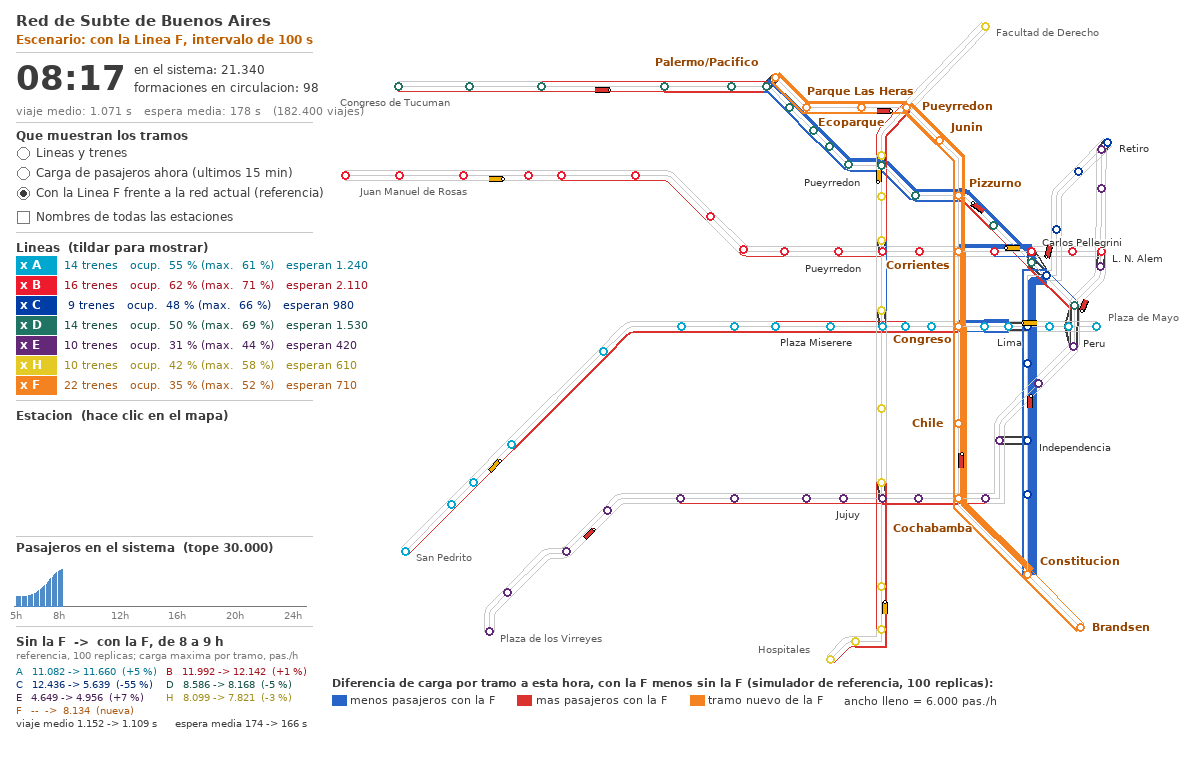
\includegraphics[width=\linewidth]{mapa-red-diferencia.png}
  \caption{Mapa de la red con la Línea F a las 8 de la mañana, mostrando cuánto cambia la carga de cada
  tramo respecto de la red sin la F: en azul los tramos que pierden pasajeros, en rojo los que ganan y en
  naranja los tramos nuevos. La Línea C se vacía entre Constitución y el centro mientras la F toma esa carga.
  A la izquierda, el reloj, los contadores por línea, la ficha de la estación elegida y la comparación de
  carga máxima por línea a esa hora.}
  \label{fig:mapa}
\end{figure}

El modelo de la red se muestra sobre un mapa con el trazado oficial (figura~\ref{fig:mapa}), dibujado con las
figuras y controles de AnyLogic. Se ven los trenes en movimiento con su ocupación y las estaciones con los
pasajeros que esperan. Los tramos se pueden colorear de tres maneras: por línea, por la carga de los últimos
quince minutos o por la diferencia entre la red con y sin la Línea F. Al hacer clic en una estación se abre
una ficha con cada uno de sus andenes.

\begin{figure}[htbp]
  \centering
  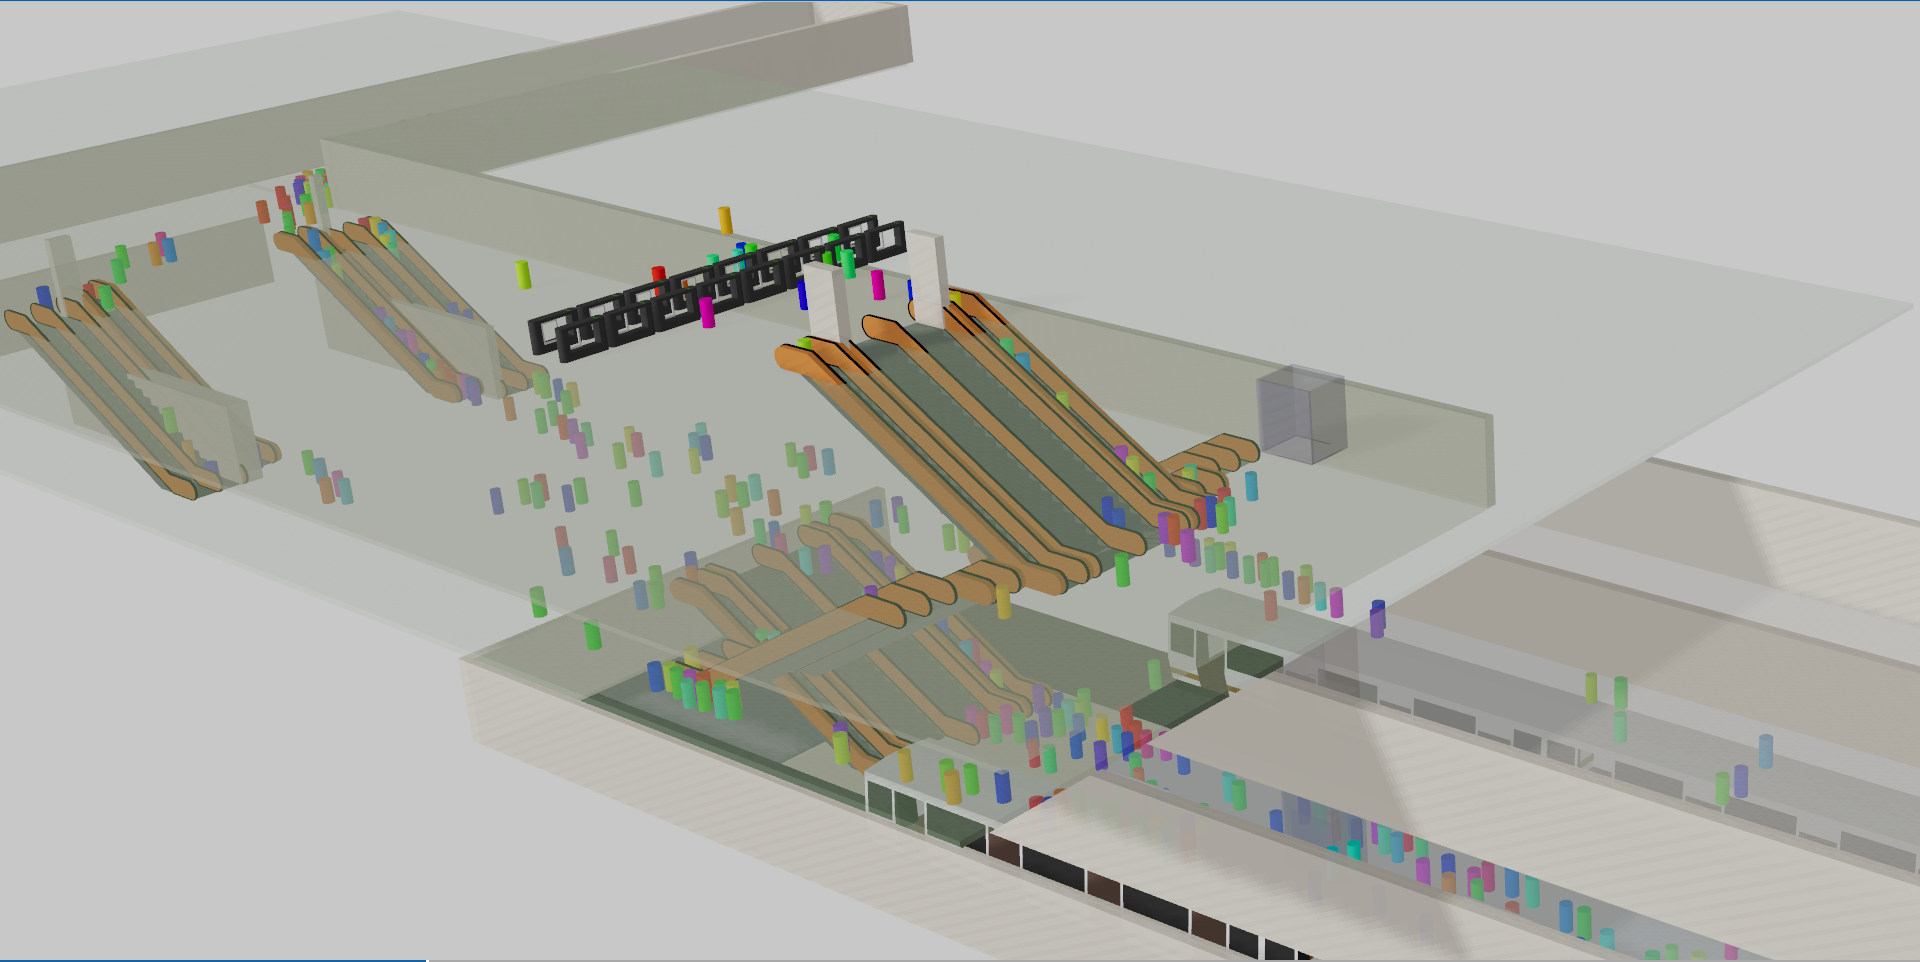
\includegraphics[width=0.49\linewidth]{3d-vista-general.png}\hfill
  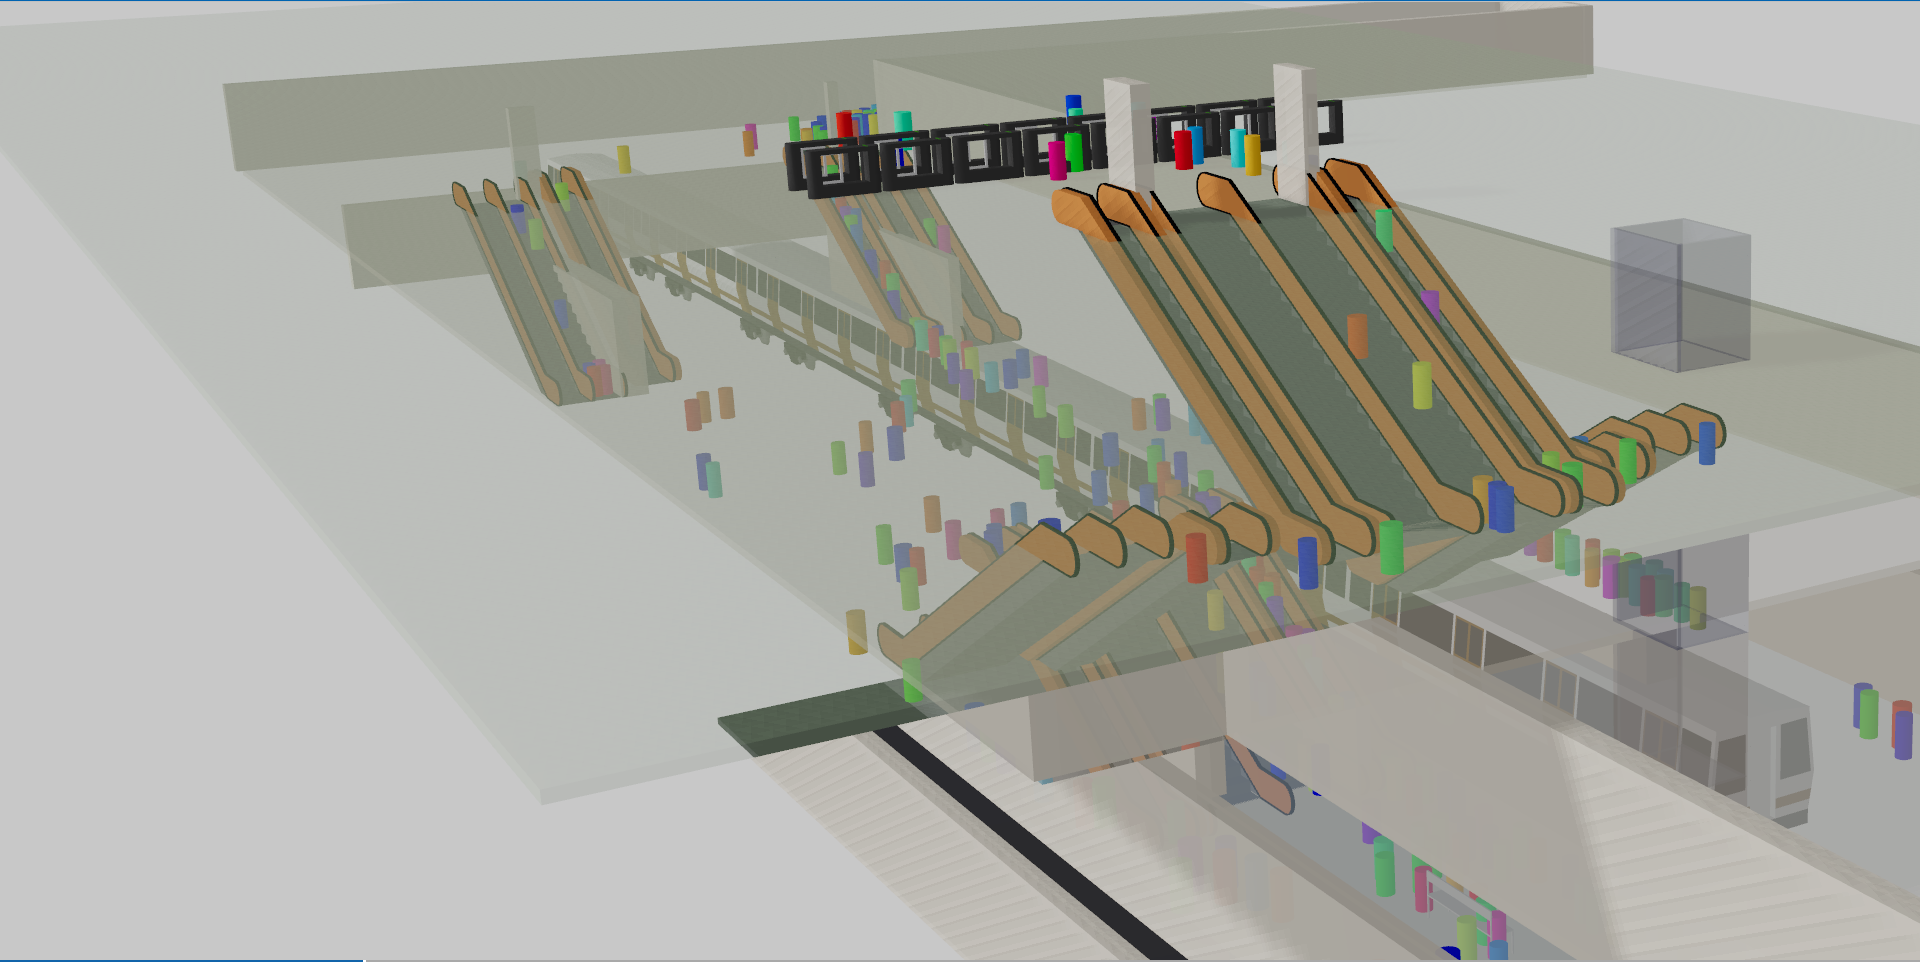
\includegraphics[width=0.49\linewidth]{3d-complejo-este.png}\\[2pt]
  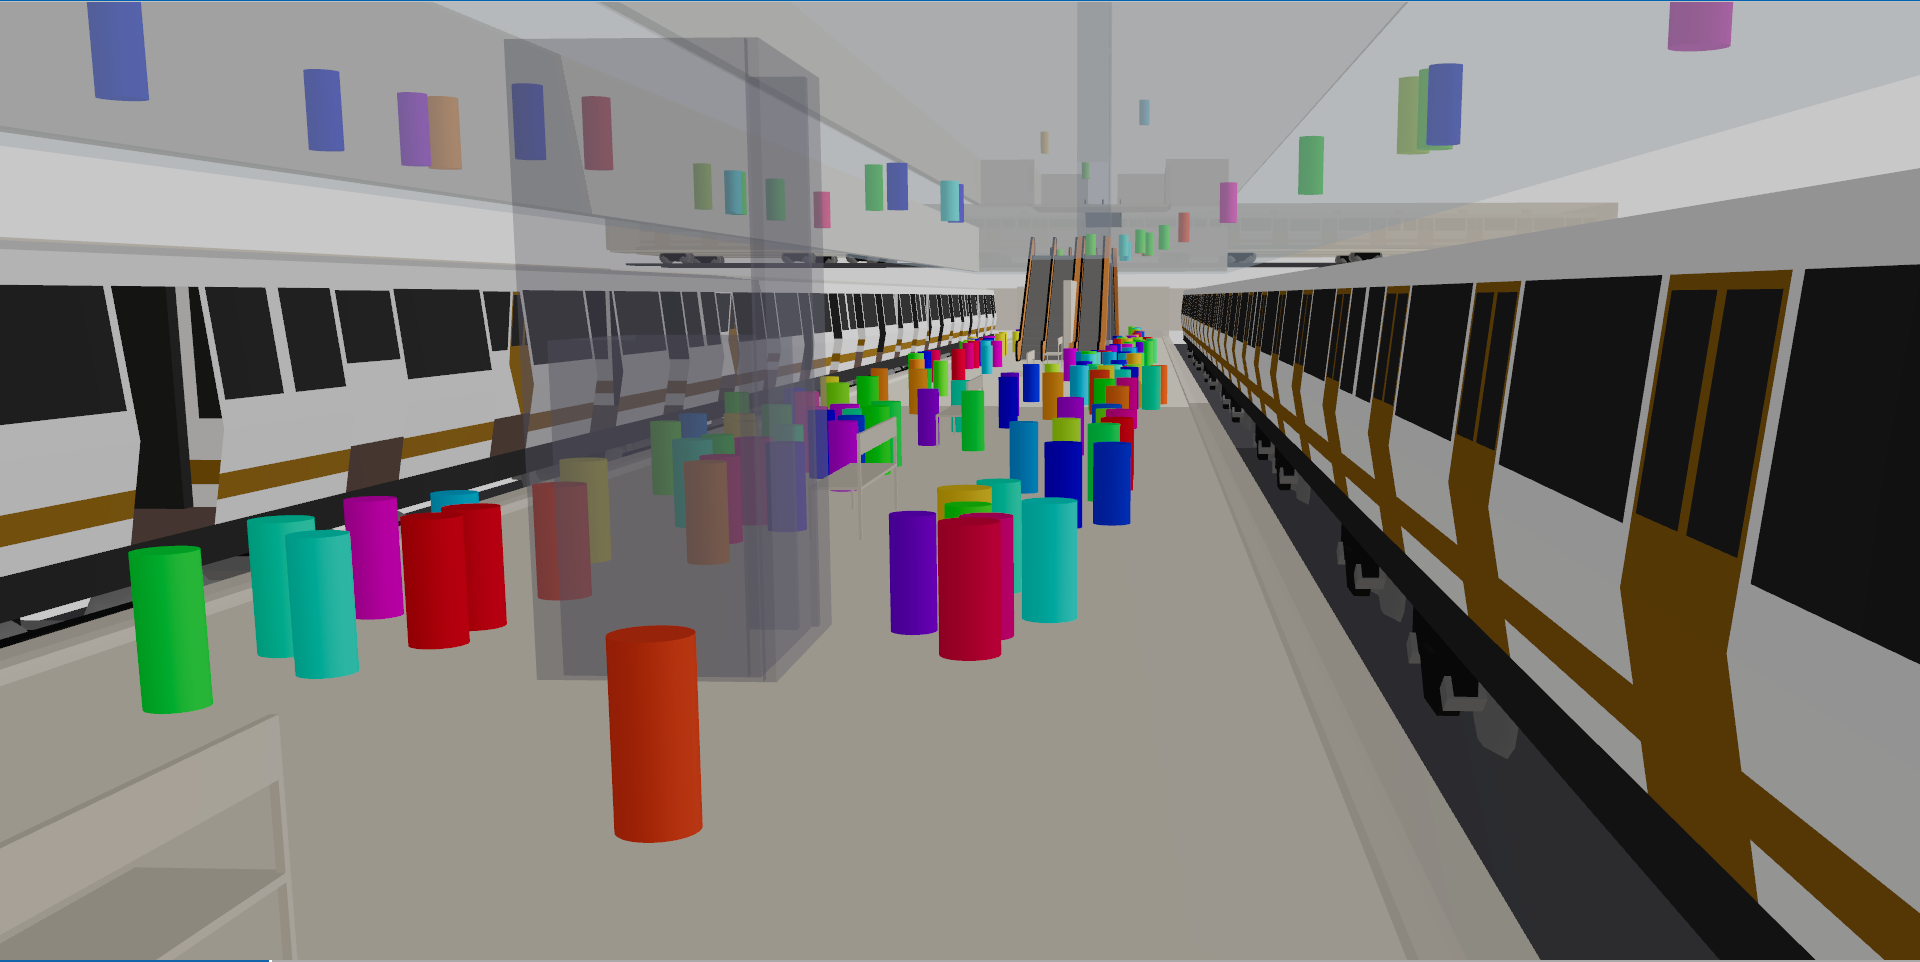
\includegraphics[width=0.49\linewidth]{3d-anden-tren.png}
  \caption{La estación Constitución de la Línea F en tres dimensiones, hora pico de la mañana. Arriba a la
  izquierda, vista general con el vestíbulo, las escaleras y la estación actual de la Línea C al fondo;
  arriba a la derecha, el complejo de escaleras del lado del Roca entre el vestíbulo y el entrepiso; abajo,
  el andén con un tren detenido. Los cilindros son los pasajeros.}
  \label{fig:3d}
\end{figure}

La estación Constitución se muestra en tres dimensiones (figura~\ref{fig:3d}), con cámaras fijas, botones
para ocultar cada nivel y trenes que llegan y parten en el mismo momento que en la simulación. Se ve también
la estación actual de la Línea C con el pasillo que la une a la F, por donde caminan los pasajeros que
combinan.

% =====================================================================
\section{Resultados}
\label{sec:resultados}

La Línea F alivia la Línea C a menos de la mitad y mejora poco el viaje promedio de la red; la estación
Constitución de la nueva línea alcanza para sus pasajeros. Cada cifra es la media de las réplicas con su
intervalo de confianza del 95\,\% (sección~\ref{sec:diseno}). Las tablas de la red son del simulador de
control, que reproduce a AnyLogic (tabla~\ref{tab:cruzada}) y permite comparar los escenarios réplica a
réplica.

\subsection{La red en conjunto: una mejora moderada}

Con la Línea F cada 100 s el tiempo medio de viaje de la red baja de 1.111 a 1.066 s y la espera media de 188
a 177 s. Calculado réplica a réplica, el ahorro es de \textbf{44,8 $\pm$ 0,6 s en el viaje} (un 4\,\%) y de
\textbf{11,6 $\pm$ 0,6 s en la espera} (tabla~\ref{tab:sensibilidad}, primera fila): con 95\,\% de confianza
el viaje medio baja entre 44,2 y 45,4 s, y el intervalo está lejos de cero, así que la diferencia es real y no
del azar. AnyLogic, con sus propias cien réplicas por escenario, da lo mismo: 45,4 $\pm$ 0,6 s menos de viaje
y 12,0 $\pm$ 0,6 s menos de espera. Es moderada porque se promedia sobre todos los viajes, y cuatro de cada cinco no cambian de ruta. Para quienes sí pasan a
usar la Línea F, el ahorro es de 162 s por viaje.

\begin{table}[htbp]
  \centering\small
  \caption{Indicadores de la red por escenario: media e intervalo de confianza del 95\,\% (simulador de
  control, cien réplicas). La última columna es el viaje medio en AnyLogic, con diez réplicas por escenario
  y $t$ de Student.}
  \label{tab:indicadores}
  \begin{tabular}{lrrrrr}
    \toprule
    Escenario & Viaje medio (s) & Espera media (s) & Viajes que usan la F & Trenes (máx.) & Viaje, AnyLogic (s) \\
    \midrule
    Red actual     & 1.110,7 $\pm$ 0,4 & 188,5 $\pm$ 0,4 & ---       & 82  & 1.111,8 $\pm$ 1,9 \\
    Con F cada 90 s    & 1.064,7 $\pm$ 0,4 & 175,8 $\pm$ 0,4 & 21,0\,\% & 106 & 1.063,4 $\pm$ 1,4 \\
    Con F cada 100 s   & 1.065,9 $\pm$ 0,4 & 176,9 $\pm$ 0,4 & 21,0\,\% & 103 & 1.064,8 $\pm$ 1,1 \\
    Con F cada 120 s   & 1.067,9 $\pm$ 0,4 & 178,9 $\pm$ 0,4 & 20,9\,\% & 100 & 1.066,6 $\pm$ 1,0 \\
    Con F cada 150 s   & 1.070,8 $\pm$ 0,5 & 181,9 $\pm$ 0,5 & 20,7\,\% & 97  & 1.072,3 $\pm$ 0,9 \\
    Con F cada 189 s   & 1.074,3 $\pm$ 0,4 & 185,3 $\pm$ 0,4 & 20,3\,\% & 93  & 1.074,8 $\pm$ 2,0 \\
    \bottomrule
  \end{tabular}
\end{table}

La frecuencia de la Línea F casi no cambia cuánta gente la usa: entre un tren cada 90 s y uno cada 189 s,
la proporción de viajes pasa del 21,0 al 20,3\,\% (tabla~\ref{tab:indicadores}). Quienes la eligen ahorran
mucho tiempo y la espera adicional no los hace desistir. Lo que sí cambia es cuánto ganan: con trenes cada
189 s el viaje medio de la red es 9,6 s más largo que con trenes cada 90 s, una diferencia muy superior a los
márgenes de $\pm$0,4 s de cada escenario. AnyLogic muestra la misma tendencia con sus propias réplicas: el
viaje medio crece de 1.063,4 a 1.074,8 s entre los dos extremos (última columna).

Con la Línea F aumentan levemente los transbordos, porque la nueva línea se usa sobre todo para combinar:
el 46\,\% de quienes suben a ella vienen de otra línea, contra el 23 a 32\,\% en las líneas A a E.

\subsection{La Línea C: el alivio que busca el proyecto}

\begin{table}[htbp]
  \centering\small
  \caption{Pasajeros por hora en el tramo más cargado de la Línea C y de la Línea F: media e intervalo de
  confianza del 95\,\% (simulador de control, cien réplicas). La última columna es la ocupación del tren más
  lleno de la Línea F en el peor de los cien días simulados.}
  \label{tab:picos}
  \begin{tabular}{lrrrr}
    \toprule
    Escenario & Línea C & Cambio en la C & Línea F & Ocupación máx. de la F \\
    \midrule
    Red actual   & 12.436 $\pm$ 64 & ---         & ---   & ---    \\
    Con F cada 90 s  & 5.625 $\pm$ 29  & $-$54,8 $\pm$ 0,3\,\% & 8.107 $\pm$ 20 & 50\,\% \\
    Con F cada 100 s & 5.639 $\pm$ 37  & $-$54,7 $\pm$ 0,4\,\% & 8.134 $\pm$ 17 & 55\,\% \\
    Con F cada 120 s & 5.662 $\pm$ 28  & $-$54,5 $\pm$ 0,3\,\% & 8.114 $\pm$ 17 & 56\,\% \\
    Con F cada 150 s & 5.663 $\pm$ 30  & $-$54,5 $\pm$ 0,3\,\% & 8.140 $\pm$ 20 & 57\,\% \\
    Con F cada 189 s & 5.640 $\pm$ 31  & $-$54,6 $\pm$ 0,3\,\% & 8.057 $\pm$ 16 & 65\,\% \\
    \bottomrule
  \end{tabular}
\end{table}

La Línea F cumple el objetivo del proyecto. El tramo más cargado de la Línea C pasa de 12.436 $\pm$ 64 a
5.639 $\pm$ 37 pasajeros por hora con un tren cada 100 s: \textbf{baja un 54,7 $\pm$ 0,4\,\%}, a menos de la
mitad, y el intervalo es prácticamente el mismo con cualquiera de las frecuencias probadas
(tabla~\ref{tab:picos}). AnyLogic, con sus propias réplicas, da el mismo alivio: 54,3 $\pm$ 0,3\,\%
(tabla~\ref{tab:cruzada}), y con diez réplicas por frecuencia el pico de la C queda entre 5.589 y 5.696
pasajeros por hora con cualquiera de ellas. La Línea C pierde el 41\,\% de sus pasajeros del día (de 183.532 a 107.880) y la
Línea F recibe 190.671 por día, el 14\,\% de la red. Las líneas A, B, D y E ganan entre un 2 y un 9\,\% de
pasajeros, de gente que ahora combina con la F.

El andén de la Línea C en Constitución hacia Retiro es hoy el más lleno de la red: en el peor de los cien días
simulados llega a tener 2.405 personas esperando a la vez. Con la Línea F, en su peor día, tiene 917.

\subsection{Cuánta gente lleva la Línea F}

\begin{figure}[htbp]
  \centering
  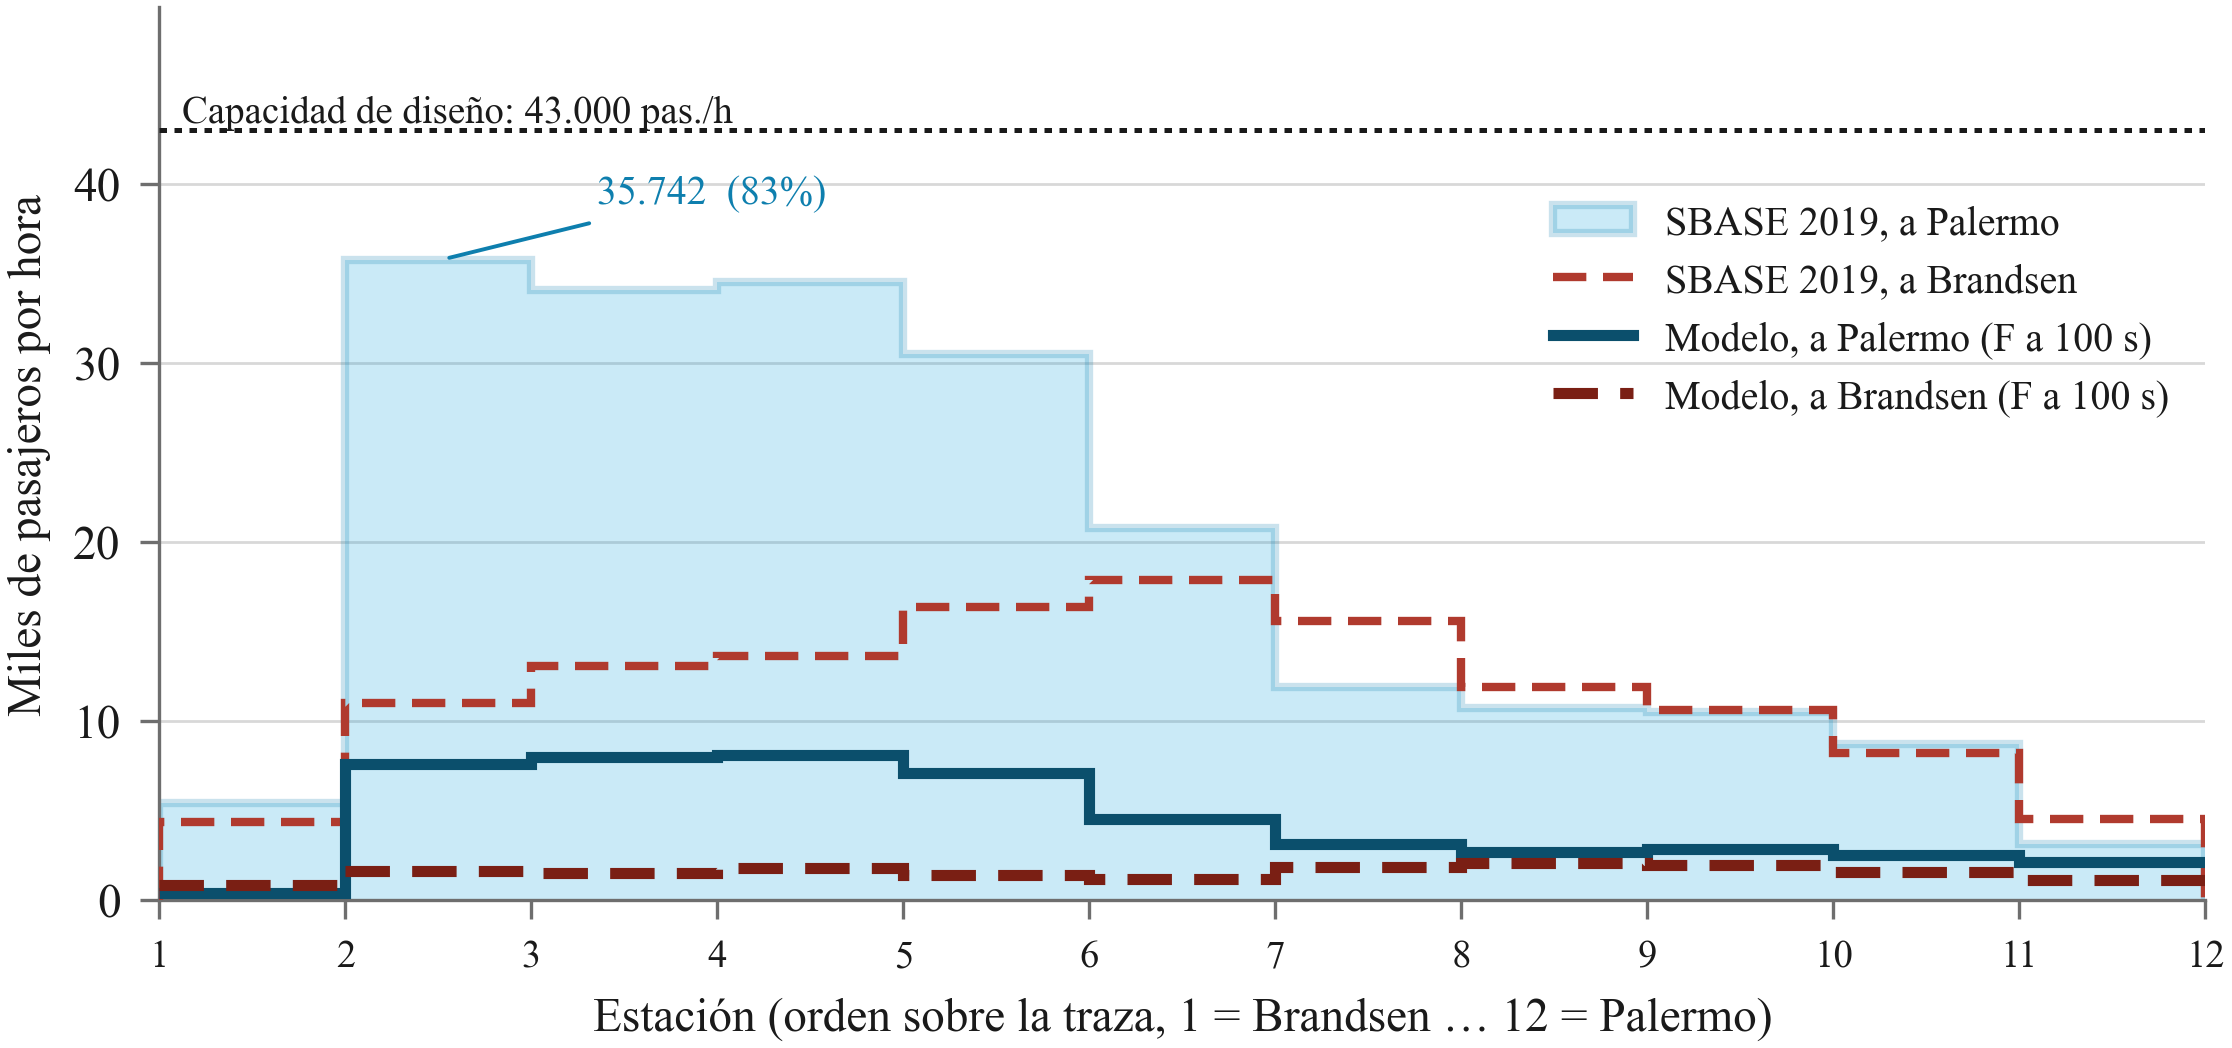
\includegraphics[width=0.9\linewidth]{perfil-carga-linea-f-modelo.png}
  \caption{Pasajeros por hora a bordo de la Línea F entre cada par de estaciones, de 8 a 9 h. En colores
  claros, lo que previó SBASE en 2019 para otra traza; en trazo oscuro, lo que da el modelo con un tren cada
  100 s. La forma es parecida en el sentido a Palermo; la cantidad, un cuarto.}
  \label{fig:perfil}
\end{figure}

En su tramo más cargado, Chile hacia Congreso de 8 a 9 h, la Línea F lleva 8.134 $\pm$ 17 pasajeros por hora.
Con un tren cada 100 s ofrece lugar para 38.664 por hora y sentido, así que ni el tren más lleno del peor de
los cien días pasa del 55\,\%:
la Línea F tiene capacidad de sobra con la demanda actual. Es un cuarto de lo que previó SBASE en 2019
(figura~\ref{fig:perfil}), y la diferencia se explica: aquel estudio sumaba pasajeros nuevos, proyectaba la
demanda a 2030 y analizaba otra traza; este modelo solo redistribuye a los pasajeros que ya existen.

\subsection{Los resultados no dependen de los supuestos}

Para comprobar que la conclusión no depende de los supuestos propios del trabajo, se cambió cada uno por una
alternativa y se repitió la comparación (tabla~\ref{tab:sensibilidad}). Las variantes fueron: repartir los
viajes a lo largo del día con una sola curva para toda la red o de manera pareja fuera de las horas pico; no
limitar la capacidad de los trenes; y hacer que el pasajero se vaya después de perder dos trenes llenos. En
todos los casos la Línea F ahorra entre 45 y 48 s de viaje medio, con márgenes de $\pm$0,6 s, y alivia la
Línea C un 54\,\%. Con el triple
de tiempo de detención por pasajero, el viaje medio cambia apenas 5 a 7 s. \textbf{La conclusión no depende de
esos supuestos.}

\begin{table}[htbp]
  \centering\small
  \caption{Efecto de la Línea F (un tren cada 100 s) con cada supuesto reemplazado por una alternativa.
  Diferencia entre los dos escenarios simulados con los mismos números al azar, intervalo de confianza del
  95\,\% (simulador de control, cien réplicas).}
  \label{tab:sensibilidad}
  \begin{tabular}{lrrr}
    \toprule
    Variante & Efecto en el viaje (s) & Efecto en la espera (s) & Efecto en el tramo pico de la C \\
    \midrule
    Supuestos del trabajo & $-$44,8 $\pm$ 0,6 & $-$11,6 $\pm$ 0,6 & $-$54,7\,\% \\
    Una sola curva horaria para la red & $-$45,3 $\pm$ 0,5 & $-$12,0 $\pm$ 0,5 & $-$54,3\,\% \\
    Viajes parejos fuera de las horas pico & $-$47,8 $\pm$ 0,6 & $-$14,2 $\pm$ 0,6 & $-$54,1\,\% \\
    Trenes sin límite de capacidad & $-$44,8 $\pm$ 0,5 & $-$11,6 $\pm$ 0,4 & $-$54,5\,\% \\
    El pasajero se va tras perder dos trenes & $-$44,9 $\pm$ 0,5 & $-$11,7 $\pm$ 0,5 & $-$54,6\,\% \\
    \bottomrule
  \end{tabular}
\end{table}

\subsection{La estación Constitución funciona en las horas pico}
\label{sec:peatonal-resultados}

La tabla~\ref{tab:peatonal} resume las diez réplicas de cada caso del submodelo (sección~\ref{sec:diseno}).

\begin{table}[htbp]
  \centering\small
  \caption{Submodelo de Constitución de la Línea F. Media $\pm$ intervalo de confianza del 95\,\% ($t$ de
  Student), diez réplicas de una hora. La mediana es el tiempo que no supera la mitad de los pasajeros; el percentil 90,
  el que no supera el 90\,\%.}
  \label{tab:peatonal}
  \begin{tabularx}{\linewidth}{>{\raggedright\arraybackslash}p{0.40\linewidth}RR}
    \toprule
    Indicador & Mañana, 8 a 9 h & Tarde, 17 a 18 h \\
    \midrule
    De la entrada al tren (s): media / mediana / percentil 90 & 167 $\pm$ 0,3 / 167 / 216 & 159 $\pm$ 0,4 / 158 / 206 \\
    Del tren a la salida (s): media / mediana / percentil 90 & 163 $\pm$ 1 / 161 / 214 & 164 $\pm$ 0,3 / 160 / 218 \\
    Personas en la estación al terminar la hora & 244 $\pm$ 13 & 60 $\pm$ 5 \\
    Escalera más cargada, lado Roca (pasajeros por hora) & 4.720 (mecánica que baja al andén) & 2.955 (mecánica que sube al vestíbulo) \\
    Si solo el 30\,\% fuera del Roca & entrada $-$3,3 $\pm$ 0,4 s ($-$2,0\,\%) & salida $-$4,0 $\pm$ 0,5 s ($-$2,4\,\%) \\
    Mecánicas del lado Roca en el sentido de la hora pico & salida $-$7,9 $\pm$ 1,3 s ($-$4,9\,\%) & salida $-$2,3 $\pm$ 1,0 s ($-$1,4\,\%; tres réplicas) \\
    Pasajeros que eligen la salida al azar & --- & salida +16,5 $\pm$ 0,4 s (+10\,\%) \\
    \bottomrule
  \end{tabularx}
\end{table}

\textbf{La estación funciona en las dos horas pico.} Las colas no crecen: al terminar la hora quedan 244
personas adentro a la mañana y 60 a la tarde, una cantidad estable. Un pasajero tarda en promedio menos de
tres minutos entre que entra y sube al tren, y lo mismo entre que baja y sale; nueve de cada diez tardan menos
de cuatro minutos.

\textbf{El punto a vigilar es el complejo de escaleras del lado del Roca.} A la mañana, su escalera mecánica
de bajada al andén mueve 4.700 pasajeros por hora: dos tercios de lo que rinde sola, sin interferencias, y
algo más de la mitad de su capacidad nominal. Tiene margen, pero es la que primero se saturaría si la
demanda creciera.

\textbf{Dos medidas sin obra mejoran la estación.} Poner las dos escaleras mecánicas de ese complejo en el
sentido de la hora pico acorta el tiempo de salida de la mañana en 7,9 $\pm$ 1,3 s (un 5\,\%). Y la
señalización importa: si los pasajeros eligieran la salida al azar en lugar de la más cercana a su destino, el
tiempo de salida de la tarde aumentaría 16,5 $\pm$ 0,4 s (un 10\,\%).

% =====================================================================
\section{Conclusiones}
\label{sec:conclusiones}

El trabajo se propuso comparar, con un modelo de simulación calibrado con datos públicos, la red de Subte
con y sin la Línea F. El modelo está construido en AnyLogic, un segundo programa hecho por separado da los
mismos resultados, y reproduce la carga real de pasajeros por tramo con un error medio del 8\,\%. Sus
respuestas son cuatro; cada cifra va con su intervalo de confianza del 95\,\%, sobre cien réplicas en la red y
diez en la estación:

\begin{enumerate}
  \item \textbf{La Línea F cumple su objetivo.} El tramo más cargado de la Línea C baja a menos de la mitad
    (54,7 $\pm$ 0,4\,\% menos, de 12.436 $\pm$ 64 a 5.639 $\pm$ 37 pasajeros por hora; AnyLogic, con sus
    propias réplicas, da 54,3 $\pm$ 0,3\,\%), y el andén de la C en
    Constitución deja de ser el más lleno de la red. El alivio es el mismo con cualquier frecuencia entre un
    tren cada 90 s y uno cada 189 s: entre 54,5 y 54,8\,\%.
  \item \textbf{Para la red en conjunto, la mejora es moderada.} El viaje medio baja 44,8 $\pm$ 0,6 s y la
    espera 11,6 $\pm$ 0,6 s, sobre un viaje de unos 18,5 minutos. Es poco en promedio porque cuatro de cada
    cinco viajes no cambian; quienes usan la Línea F ahorran casi tres minutos.
  \item \textbf{La Línea F tiene capacidad de sobra.} Con los pasajeros actuales lleva 8.134 $\pm$ 17 por hora
    en su tramo más cargado, y ni el tren más lleno del peor día simulado pasa de poco más de la mitad
    (55\,\%). Llenarla requeriría pasajeros nuevos que hoy no usan el Subte. Por eso, una frecuencia menor que
    la de diseño mantendría el alivio de la Línea C con menos trenes, a cambio de unos segundos más de espera
    (con un tren cada 189 s, el viaje medio es 9,6 s más largo que con uno cada 90 s).
  \item \textbf{La estación Constitución de la Línea F, tal como está proyectada, funciona en las horas
    pico.} Un pasajero tarda 167 $\pm$ 0,3 s en promedio en llegar al tren en la hora pico de la mañana y
    159 $\pm$ 0,4 s en la de la tarde, menos de tres minutos, sin colas que crezcan. El complejo de
    escaleras del lado del Roca es el punto a vigilar, y dos medidas sin obra lo mejoran: operar sus escaleras
    mecánicas en el sentido de la hora pico y señalizar bien las salidas.
\end{enumerate}

Sobre el método, lo que más pesó fueron los datos. Conseguir la matriz de viajes por pedido de acceso a la
información, y encontrar y corregir los errores de las fuentes oficiales, cambió más el resultado que
cualquier decisión de modelado.

\subsection{Limitaciones}
\label{sec:limitaciones}

\begin{itemize}
  \item \textbf{La demanda de la Línea F se construyó en el modelo.} Incluye a los pasajeros actuales que
    cambian de ruta y a los nuevos de las estaciones sin combinación, pero no a quienes empezarían a usar el
    Subte por la nueva línea. Por eso la carga de la F es menor que la prevista por SBASE en 2019, que sí los
    contaba. Las dos previsiones oficiales se contradicen y el trabajo no puede decidir cuál es la correcta.
  \item \textbf{La demanda es de un día.} La matriz de SBASE es un día hábil de septiembre de 2024; fuera de
    las horas pico, el reparto horario sale de una encuesta con destinos estimados. Las pruebas de
    sensibilidad muestran que el resultado no depende de ese reparto.
  \item \textbf{Cada pasajero usa una sola ruta}, la más rápida. Retiro tiene un error conocido en el reparto
    entre las líneas C y E.
  \item \textbf{La espera y la gente en los andenes no se pueden contrastar} con ningún dato observado. Valen
    para comparar escenarios.
  \item \textbf{Los trenes salen de cada cabecera sin coordinación entre sí} y sin límite de flota: el modelo
    no reproduce que un tren atrasado suele atrasar al siguiente.
  \item \textbf{Submodelo de Constitución.} La velocidad de marcha es algo mayor que la media bibliográfica,
    así que los tiempos son optimistas; la capacidad del tren no se modela; los molinetes y la estación de la C
    quedan fuera del cálculo.
  \item \textbf{Alcance.} El Premetro queda fuera. Las líneas del corredor de la Línea F (A, C, D y H) se
    calibraron con más detalle que la B y la E.
\end{itemize}

% =====================================================================
\section*{Referencias}
\begin{list}{}{\leftmargin=2em \itemindent=-2em \itemsep=0.25em}

\item[] [1] Neirotti, B., Galasco, A., Salami, T., Mesapelle, G. y Lovatti, F. (2026).
  \textit{Propuesta de TPI de Simulación: Evaluación del impacto de la Línea F sobre la operación de la red
  de Subte de la Ciudad de Buenos Aires}. UTN FRRo, agosto de 2026.

\item[] [2] Law, A. M. (2015). \textit{Simulation Modeling and Analysis} (5.\textsuperscript{a} ed.).
  McGraw-Hill Education.

\item[] [3] Ortúzar, J. de D. y Willumsen, L. G. (2011). \textit{Modelling Transport} (4.\textsuperscript{a}
  ed.). John Wiley \& Sons.

\item[] [4] Subterráneos de Buenos Aires (SBASE). \textit{Subte: Viajes Molinetes}. Buenos Aires Data.
  Archivos anuales, 2013--2025. \url{https://data.buenosaires.gob.ar/dataset/subte-viajes-molinetes}

\item[] [5] Subterráneos de Buenos Aires (SBASE). \textit{Subte: Trenes despachados}. Buenos Aires Data.
  Recursos anuales 2024, 2025 y 2026. \url{https://data.buenosaires.gob.ar/dataset/subte-trenes-despachados}

\item[] [6] Subterráneos de Buenos Aires (SBASE). \textit{Subte: GTFS}. Buenos Aires Data. Versión 2.0.
  \url{https://data.buenosaires.gob.ar/dataset/subte-gtfs}

\item[] [7] Subsecretaría de Planificación de la Movilidad y Seguridad Vial. \textit{Viajes y etapas en
  transporte público del Área Metropolitana de Buenos Aires 2019 a 2024}. Buenos Aires Data.
  \url{https://data.buenosaires.gob.ar/dataset/viajes-etapas-transporte-publico}

\item[] [8] Observatorio de Movilidad y Seguridad Vial de la Ciudad de Buenos Aires. \textit{Dataset de
  Viajes y Etapas en Transporte Público del Área Metropolitana de Buenos Aires. Notas para su uso,
  2019--2025}. Abril de 2025.

\item[] [9] Gobierno de la Ciudad Autónoma de Buenos Aires. \textit{Respuestas a las Solicitudes de Acceso a
  la Información Pública, Ley 104, N.\textsuperscript{o} 00866317/26 y 00934682/26}. Se citan en particular
  IF-2026-38553261-GCABA-SBASE (matriz origen--destino y perfiles de carga por tramo, EMOVA S.A., septiembre de
  2024), IF-2026-37530623-GCABA-MMIGC (distancias entre estaciones, intervalo de diseño, tiempo entre
  cabeceras, composición de las formaciones, etapas de habilitación) e IF-2019-20550252-GCABA-SBASE
  (\textit{Análisis de Demanda Línea F}, SBASE, 2019).

\item[] [10] Agencia de Protección Ambiental, GCBA. \textit{Estudio de Impacto Ambiental, Proyecto «Línea
  F -- Sistema Integrado de Movilidad»}. Expediente EX-2026-20211143-GCABA-APRA, 98 documentos. Capítulo 3,
  \textit{Descripción del proyecto} (parámetros operativos, estaciones y progresivas) y capítulo 6,
  \textit{Estudios especiales} (Línea C y PETERS; pasajeros por estación).

\item[] [11] Gobierno de la Ciudad Autónoma de Buenos Aires, Ministerio de Movilidad e Infraestructura.
  \textit{Licitación pública N.\textsuperscript{o} 10241-0094-LPU25, «Ingeniería, construcción y
  equipamiento línea de Subterráneo F»}. Portal BA Obras. Pliego de Cláusulas Particulares, Pliego de
  Especificaciones Técnicas (sección 19, escaleras mecánicas), planos de la estación Constitución y
  Resolución 175/GCABA-MMIGC/26. \url{https://buenosairesobras.dguiaf-gcba.gov.ar}

\item[] [12] Legislatura de la Ciudad Autónoma de Buenos Aires. \textit{Ley 670}, 8 de noviembre de 2001.

\item[] [13] Subterráneos de Buenos Aires y Banco Interamericano de Desarrollo. \textit{Plan Estratégico y
  Técnico para la Expansión de la Red de Subtes de Buenos Aires (PETERS)}. AC\&A, 2015.

\item[] [14] Transportation Research Board (2013). \textit{Transit Capacity and Quality of Service Manual}
  (3.\textsuperscript{a} ed.), TCRP Report 165. Tiempos de ascenso y descenso por pasajero.

\item[] [15] Fruin, J. J. (1971). \textit{Pedestrian Planning and Design}. Metropolitan Association of
  Urban Designers and Environmental Planners.

\item[] [16] Weidmann, U. (1993). \textit{Transporttechnik der Fussgänger}. Schriftenreihe des IVT 90, ETH
  Zürich.

\item[] [17] Zacharias, J. y Tang, Y. (2015). Escalator versus stairs choice in urban rail stations.
  \textit{Transportation Research Procedia}, citado para la preferencia por la escalera mecánica.

\item[] [18] Pouw, C., Corbetta, A., Gabbana, A., van der Laan, C. y Toschi, F. (2024). \textit{High-statistics
  pedestrian dynamics on stairways and their probabilistic fundamental diagrams}. arXiv:2307.15609. Diagramas
  fundamentales de Fruin y de Predtechenskii y Milinskii para escaleras.

\item[] [19] The AnyLogic Company. \textit{AnyLogic 8.9 Personal Learning Edition}, Process Modeling Library y
  Pedestrian Library. Documentación en \url{https://anylogic.help}

\item[] [20] Ross, S. M. (1999). \textit{Simulación} (2.\textsuperscript{a} ed.). Prentice Hall. Traducción de la
  segunda edición en inglés, \textit{Simulation} (Academic Press). Capítulo 7, \textit{Análisis estadístico de
  datos simulados}: secciones 7.1, \textit{Media y varianza muestrales}, y 7.2, \textit{Estimación del
  intervalo de una media poblacional}.

\item[] [21] Ross, S. M. (2013). \textit{Simulation} (5.\textsuperscript{a} ed.). Academic Press. Capítulo 8,
  \textit{Statistical Analysis of Simulated Data}: secciones 8.1 y 8.2, las mismas 7.1 y 7.2 de la edición en
  castellano, con el mínimo de datos llevado de 30 a 100.

\item[] [22] EMOVA Movilidad S.A. y Subterráneos de Buenos Aires. \textit{Subte: mapa de red} (esquemático
  oficial), 2025. Versión vectorial para la web.

\end{list}

% =====================================================================
\appendix
\section{Supuestos del modelo}
\label{sec:anexo}

\subsection*{Modelo de la red}

\begin{itemize}
  \item \textbf{Demanda.} La cantidad de viajes y su reparto entre estaciones salen de la matriz de SBASE; las
    dos horas pico, de sus matrices de hora pico; el resto del día, del perfil horario de la encuesta de
    destinos. Se conservan los viajes que la encuesta marca como incompletos (4,1\,\%), porque no cambian el
    total ni las horas pico. La demanda se modela por estación y no por andén: solo el 70,5\,\% de los
    registros de molinetes permite saber el andén.
  \item \textbf{Rutas.} Cada pasajero usa la ruta más rápida, con 120 s de penalización por transbordo. Hay
    142 rutas hacia Alberti o desde Pasco, en la Línea A, que tienen un andén para un solo sentido y obligan
    a ir y volver; se dejaron como están.
  \item \textbf{Trenes.} Intervalos sorteados de la distribución empírica de cada línea, cabecera y hora
    (julio a diciembre de 2025), sin los cortes de servicio ni los trenes cancelados con causa registrada.
    Al abrir, los trenes arrancan desde donde arrancan en la realidad. No hay tope de flota.
  \item \textbf{Andén y detención.} Quien no entra en un tren espera el siguiente. La detención es de 24 s
    (30 s en la Línea F) más el tiempo de bajada y subida del TCQSM [14]. Un tren no entra a un tramo ocupado.
  \item \textbf{Fuentes con defectos.} Un sentido de la Línea E del GTFS se reemplazó por el contrario. El
    reparto entre San Pedrito y San José de Flores, mal cargado en la encuesta de destinos, no afecta al
    modelo porque la demanda sale de la matriz de SBASE.
  \item \textbf{Calibración.} Con más detalle en el corredor de la Línea F y las líneas con las que combina.
\end{itemize}

\subsection*{Escenario con la Línea F}

\begin{itemize}
  \item La frecuencia es una variable: 90, 100, 120, 150 y 189 s, con un mínimo técnico de 90 s.
  \item Sus pasajeros son los que cambian de ruta más los de las cinco estaciones sin combinación, estimados
    con sus tres estaciones vecinas más cercanas, ponderadas por el inverso del cuadrado de la distancia y sin
    contar las terminales ferroviarias. Sin demanda inducida.
  \item Combina en las seis estaciones del expediente y con la Línea H en Pueyrredón. Subir a la F cuesta,
    al elegir la ruta, la mitad de su intervalo.
\end{itemize}

\subsection*{Submodelo de Constitución}

\begin{itemize}
  \item La geometría sigue los planos de la licitación con la mayor fidelidad posible; la estación actual de
    la Línea C se relevó a distancia, con información pública.
  \item El 70\,\% de los pasajeros va o viene del Roca; el 30\,\% se probó como alternativa.
  \item Preferencia por la escalera mecánica: 75\,\% al subir y 67\,\% al bajar [17]. En cada par de mecánicas
    una sube y otra baja; poner las dos en el sentido de la hora pico se probó como medida.
  \item Quien baja del tren toma la escalera más cercana a su destino. Para bajar al andén se elige el
    complejo del lado del Roca salvo que tenga más de 60 personas en cola.
  \item Velocidad de marcha entre 1,5 y 1,75 m/s, por encima de los 1,34 a 1,35 m/s que miden Fruin [15] y
    Weidmann [16]: representa al pasajero habitual de hora pico y da tiempos optimistas.
  \item Se puede subir al tren hasta que cierra las puertas, 30 s después de llegar. Los trenes de las dos
    vías llegan desfasados medio intervalo.
  \item La escalera fija conserva la capacidad que trae la biblioteca, mayor que la de la bibliografía [18];
    no condiciona los resultados porque trabaja a menos de un cuarto de esa capacidad.
  \item Los molinetes, la estación de la Línea C y el pasillo que las une se muestran en la animación pero
    no entran en el cálculo.
\end{itemize}

\subsection*{Modelos de AnyLogic}

\texttt{RedSubte\_mapa} es el modelo de la red con el mapa animado; el parámetro \texttt{escenario} elige la
red actual o la Línea F a cada intervalo. \texttt{RedSubte\_red} es el mismo modelo sin animación, con los
experimentos de réplicas y de variación de la frecuencia. \texttt{ConstitucionF\_3D} es la estación en tres
dimensiones; los resultados de la tabla~\ref{tab:peatonal} salen de las versiones sin animación del mismo
submodelo. Los dos modelos de la red leen sus tablas de la carpeta \texttt{datos} de
\texttt{RedSubte\_mapa}, generadas a partir de las fuentes públicas citadas; el submodelo trae sus pasajeros
dentro del propio proyecto.

\end{document}
